%%%%%%%%%%%%%%%%%%%%%%%%%%%%% Define Article %%%%%%%%%%%%%%%%%%%%%%%%%%%%%%%%%%
\documentclass{article}
%%%%%%%%%%%%%%%%%%%%%%%%%%%%%%%%%%%%%%%%%%%%%%%%%%%%%%%%%%%%%%%%%%%%%%%%%%%%%%%

%%%%%%%%%%%%%%%%%%%%%%%%%%%%% Using Packages %%%%%%%%%%%%%%%%%%%%%%%%%%%%%%%%%%
\usepackage{listings, xcolor}
\usepackage{parskip}
\usepackage{hyperref}
\usepackage{amsmath}
\usepackage{graphicx}
\usepackage[a4paper, margin = 1.5cm]{geometry}
\usepackage{float}
\usepackage{amsmath}
\usepackage{amssymb}
\usepackage{parskip}
\usepackage{listings}
\usepackage{physics}

\lstset{
frame = shadowbox,
basicstyle = \small\ttfamily,
mathescape = true,
numbers = left,
commentstyle = \itshape\color{gray}
columns = flexible,
keepspaces = true,
moredelim = [l]{//}
}

%%%%%%%%%%%%%%%%%%%%%%%%%%%%%% Title & Author %%%%%%%%%%%%%%%%%%%%%%%%%%%%%%%%
\title{Riassunto Social Computing}
\author{Trentin Tommaso}
%%%%%%%%%%%%%%%%%%%%%%%%%%%%%%%%%%%%%%%%%%%%%%%%%%%%%%%%%%%%%%%%%%%%%%%%%%%%%%
\begin{document}
\maketitle
\tableofcontents
\newpage

\section{Social media}
  Tecnologie che facilitano \textbf{creazione} e \textbf{condivisione} di informazioni, idee, interessi e altre forme di espressione mediante \textbf{community virtuali} e \textbf{network}.
  \begin{itemize}
      \item Applicazioni internet-based \textbf{Web 2.0};
      \item Sviluppate avendo come scopo principale la gestione di \textbf{User-generated content};
      \item Utenti creano \textbf{profili} e identità service-specific che vengono mantenuti dalla social media organization;
      \item Facilitano lo sviluppo di \textbf{social network online} connettendo il profilo di un utente con quello di altri individui / organizzazioni.
  \end{itemize}

  \subsection{Classificazione}
    2 dimensioni principali: \textbf{Social presence / Media richness} (quanto sembra di essere "lì") e \textbf{Self presentation / Self disclosure} (quanto si rivela di sé).
    \begin{figure}[H]
        \centering
        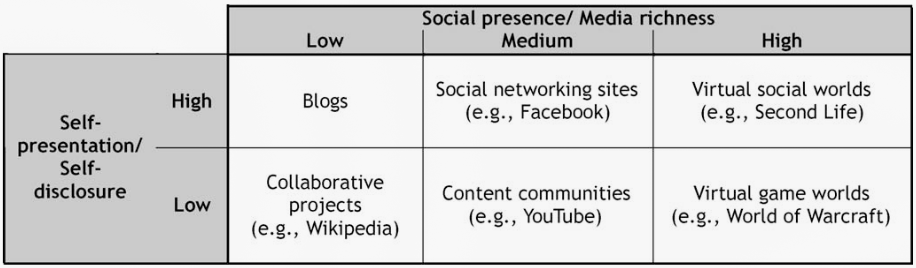
\includegraphics[width=0.6\linewidth]{figures/sm_cla.png}
    \end{figure}
    Visione articolata:
    \begin{figure}[H]
        \centering
        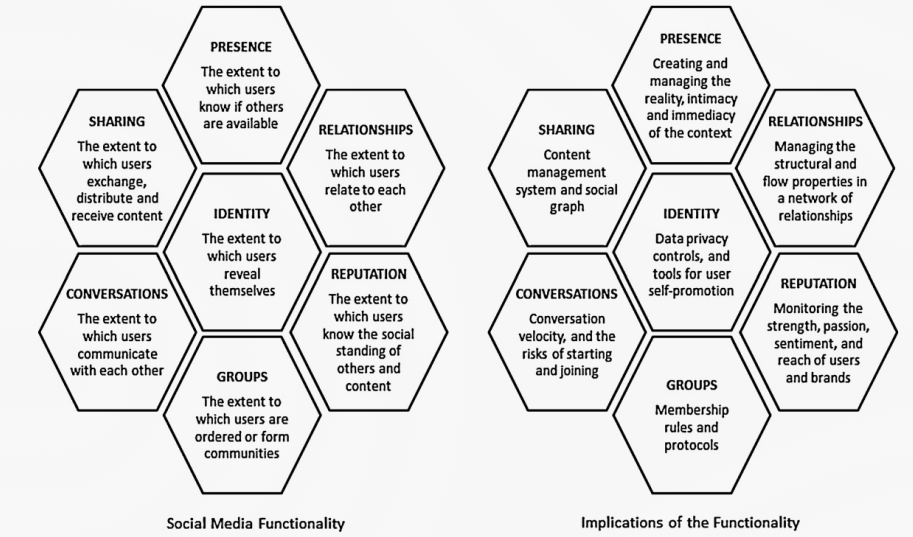
\includegraphics[width=0.5\linewidth]{figures/sm_cla_alt.png}
    \end{figure}

\section{Grafi e Reti}
  \subsection{Nodi vs. Attori (dipende dal contesto)}
    $$V={v_1,v_2,...,v_n}$$
    \begin{itemize}
        \item Grafo del Web:
           \begin{itemize}
               \item Nodi = pagine/siti web;
               \item Archi = link ipertestuali.
           \end{itemize}
        \item Grafo sociale di amicizie:
          \begin{itemize}
               \item Nodi = persone;
               \item Archi = amicizie, conoscenze...
          \end{itemize}
    \end{itemize}
    \textbf{Grandezza del grafo} (size): $\abs{V}=n$
  \subsection{Archi}
    $$E={e_1,e_2,...,e_m}$$
    Gli archi (edges) connettono nodi (ties / relationships). In un settng sociale:
    \begin{itemize}
        \item Nodi = entità sociali (persone);
        \item Archi = relazioni fra persone;
    \end{itemize}
    \textbf{Grandezza dell'insieme degli archi}: $\abs{E}=m$
  \subsection{Grafi}
    Un grafo \textit{G} si può rappresentare come coppia dell'insieme di nodi \textit{V} e archi \textit{E}:
    $$G(V,E)$$
    \subsubsection{Proprietà}
      \begin{itemize}
          \item Archi possono avere direzioni ($e(v_1,v_2) \neq e(v_2,v_1)$);
          \item \textbf{Grafo pesato}: ad ogni arco è associato un peso ($G(V,E,W)$);
          \item Grafo $G'(V',E')$ è \textbf{sottografo} di $G(V,E)$ se ($V' \subseteq V$) e ($E' \subseteq (V' \times V') \cap E$);
          \item \textbf{Vicinato} di un nodo: tutti i nodi ad esso collegati mediante archi (incoming / outgoing neighbors);
          \item \textbf{Cammino}: sequenza di archi t.c. ogni arco è incidente allo stesso nodo del successivo;
          \item \textbf{Connessione}:
            \begin{itemize}
                \item Un \textbf{nodo} $v_i$ è connesso al nodo $v_j$ se esiste cammino da $v_i$ a $v_j$ (e viceversa);
                \item Un \textbf{grafo} è connesso se esiste un cammino fra ogni coppia di nodi (\textit{fortemente} se il cammino è diretto, \textit{debolmente} altrimenti)
            \end{itemize}
          \item \textbf{Componenti}:
            \begin{itemize}
                \item \textbf{Componente in un grafo indiretto}: è un sottografo massimale connesso.
                \begin{itemize}
                    \item Esiste un cammino indiretto fra ogni coppia di nodi nella componente.
                    \item \textit{"Massimale"} significa che se si aggiungono altri nodi del grafo originale, il sottografo non è più connesso.
                \end{itemize}
                \item \textbf{Componente Fortemente Connessa} (Strongly Connected Component, \textbf{SCC}): In un grafo diretto, si ha una SCC quando per ogni coppia di nodi $u, v \in \text{SCC}$ esiste un cammino \textit{diretto} da $u$ a $v$ e uno da $v$ a $u$.
                \item \textbf{Componente Debolmente Connessa} (Weakly Connected Component, \textbf{WCC}): In un grafo diretto, si ha una WCC quando per ogni coppia di nodi $u, v \in \text{WCC}$ esiste un cammino \textit{indiretto} da $u$ a $v$.
                \item Un grafo può avere diverse componenti (ne ha solo 1 se l'intero grafo è connesso).
                \item \textbf{Giant Connected Component}: è la componente più grande del grafo e contiene "quasi tutto" il grafo (la maggior parte dei nodi).
            \end{itemize} 
      \end{itemize}
  \subsection{Gradi}
    $\pi(d)={d_1,d_2,...,d_n}$
    \textbf{Grado di un nodo $i$} $d_i$: numero di archi collegati a quel nodo (entranti = \textbf{in-degree} $d^{in}_i$, uscenti = \textbf{out-degree} $d^{out}_i$).
    \\
    \textbf{Degree distribution}: per ogni nodo, quanti nodi hanno quel grado:
    $$p_{grado}=\frac{numNodi_{grado}}{numNodi}, \sum_{d=0}^{\infty}p_{grado}=1$$
    \\
    \textbf{Teorema}: sommatoria dei gradi di un grafo indiretto è 2 volte il numero degli archi
    $$\sum_id_i=2\abs{E}$$
    \textbf{Corollari}:
    \begin{enumerate}
        \item numero di nodi con grado dispari è pari;
        \item in ogni grafo diretto la sommatoria degli in-degree è uguale alla somma degli out-degree
    \end{enumerate}
    $$\sum_id^{out}_i=\sum_jd^{in}_j$$
    \begin{figure}[H]
        \centering
        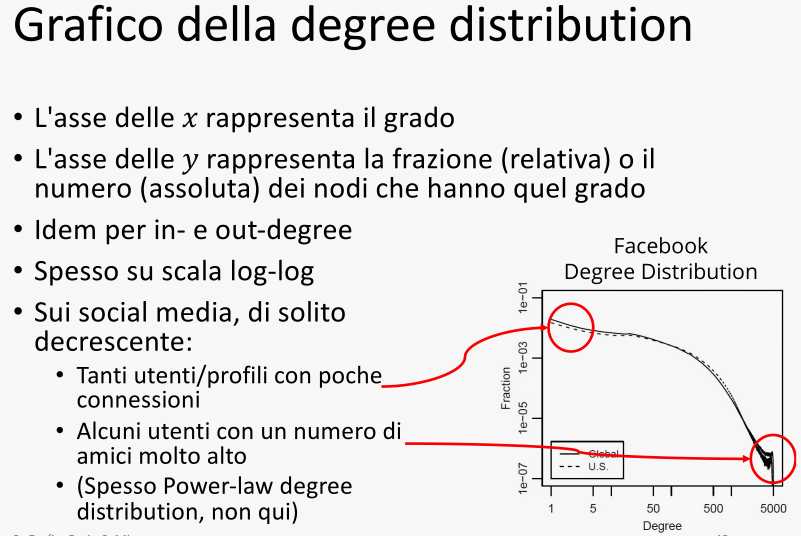
\includegraphics[width=0.5\linewidth]{figures/deg_distr.png}
    \end{figure}
  \subsection{Densità}
    Quanti archi ci sono rispetto a tutti gli archi possibili:
    \begin{itemize}
      \item Grafi \textbf{indiretti} - $D=\frac{2\abs{E}}{\abs{V}(\abs{V}-1)}$
      \item Grafi \textbf{diretti} - $D=\frac{\abs{E}}{\abs{V}(\abs{V}-1)}$
    \end{itemize}
  \subsection{Rappresentazioni}
    \subsubsection{Lista degli archi}
      \begin{itemize}
          \item Ogni elemento della lista è un arco da un nodo u a un nodo v $(u,v)$;
          \item Ok anche per grafi diretti; 
          \item Non ok per nodi isolati: non vengono rappresentati.
      \end{itemize}
      \begin{figure}[H]
          \centering
          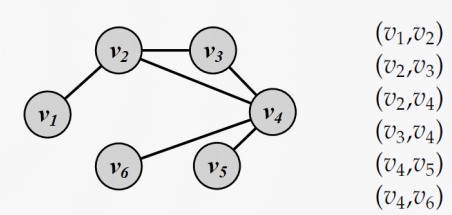
\includegraphics[width=0.5\linewidth]{figures/l_ar.png}
      \end{figure}
    \subsubsection{Lista di adiacenza}
      \begin{itemize}
          \item Per ogni nodo, lista di tutti i nodi a cui è connesso;
          \item Solitamente ordinata;
          \item Ok anche per grafi diretti.
      \end{itemize}
      \begin{figure}[H]
          \centering
          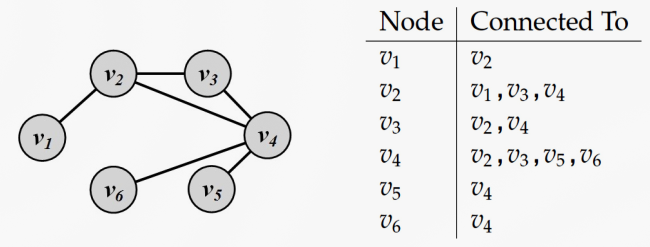
\includegraphics[width=0.5\linewidth]{figures/l_ad.png}
      \end{figure}
    \subsubsection{Matrice di adiacenza}
      \begin{itemize}
          \item Quadrata (1 se c'è un arco fra $v_i$ e $v_j$, 0 altrimenti);
          \item Simmetrica per grafi indiretti;
          \item Ok per grafi diretti (generalmente non simmetrica);
          \item Auto-archi (self-link) sulla diagonale;
          \item Per reti sociali le matrici di adiacenza sono sparse (quasi tutti 0);
          \item Ok per grafi pesati ()
          \item Quadrata ($w_{ij}$ se c'è un arco fra $v_i$ e $v_j$, 0 altrimenti);
      \end{itemize}
      \begin{figure}[H]
          \centering
          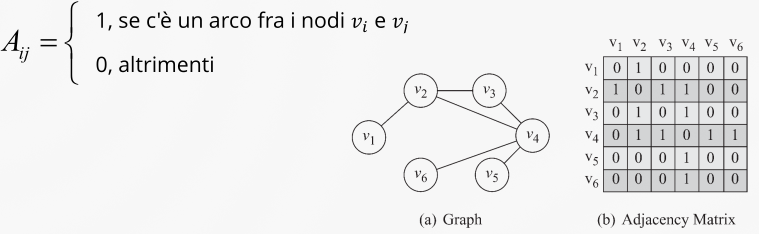
\includegraphics[width=0.5\linewidth]{figures/mat_ad.png}
      \end{figure}
  \subsection{Reti}
    Una rete (\textbf{network}) è un grafo (solitamente grande) con nodi e archi che esistono nel mondo reale, solitamente per rappresentare problemi su una rete si usano grafi e risultati della teoria dei grafi.
    \subsubsection{Reti sociali}
      Reti i cui elementi hanno una struttura sociale:
      \begin{itemize}
          \item Insieme di \textbf{attori} = individui / organizzazioni;
          \item Insieme di \textbf{legami} = connessioni fra attori.
      \end{itemize}
      Esempi: rete di familiari / amici / colleghi.
    \subsubsection{Analisi delle reti sociali (Social Network Analysis - SNA)}
      Settore interdisciplinare (scienze sociali + statistica + teoria dei grafi + reti complesse + informatica) che studia queste reti.
\section{Reti e Misure}
  \subsection{Centralià}
    \textbf{Misura} che indica quanto un nodo è centrale, basandosi su definizioni / assunzioni.
    \subsubsection{Centralità di grado}
      Più è alto il grado di un nodo, più è centrale.
      $$C_d(v_i)=d_i$$
      \begin{figure}[H]
          \centering
          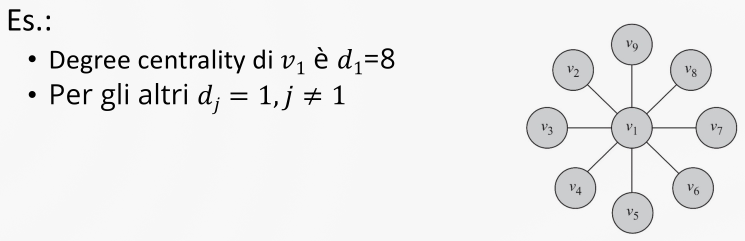
\includegraphics[width=0.6\linewidth]{figures/deg_cen.png}
      \end{figure}
      In grafi diretti si possono usare in-degree, out-degree o combinazione dei due:
      \begin{itemize}
        \item $C_d(v_i)=d^{in}_i$ (prestige);
        \item $C_d(v_i)=d^{out}_i$ (gregariousness);
        \item $C_d(v_i)=d^{in}_i+d^{out}_i$.
      \end{itemize}
      In pratica in-degree è il più usato / interessante.
    \subsubsection{Centralità di grado normalizzata}
      Utile per confrontare grafi differenti:
      \begin{itemize}
        \item Normalizzazione per grado massimo possibile - $C^{norm}_d(v_i)=\frac{d_i}{n-1}$;
        \item Normalizzazione per grado massimo effettivo - $C^{max}_d(v_i)=\frac{d_i}{max_jd_j}$;
        \item Normalizzazione per somma dei gradi - $C^{sum}_d(v_i)=\frac{d_i}{\sum_jd_j}=\frac{d_i}{2\abs{E}}=\frac{d_i}{2m}$.
      \end{itemize}
      \begin{figure}[H]
          \centering
          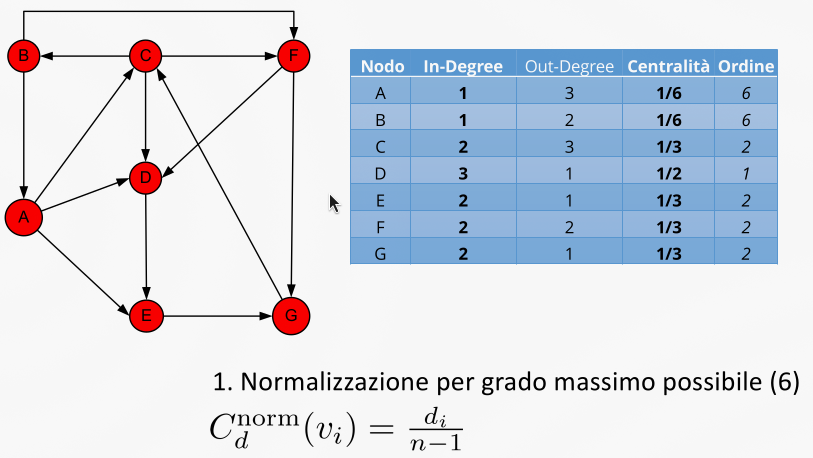
\includegraphics[width=0.5\linewidth]{figures/deg_cen_n.png}
      \end{figure}
    \subsubsection{Betweenness centrality}
      Misura quanto un nodo è importante nel connettere altri nodi tramite cammini (si guradano solo shortest paths).
      $$C_b(v_i)=\sum_{s\neq t\neq v_i}\frac{\sigma_{st}(v_i)}{\sigma_{st}}$$
      \begin{itemize}
        \item $\sigma_{st}(v_i)$: numero di shortest paths da $s$ a $t$ che passano per $v_i$;
        \item $\sigma_{st}$: nuemero di shortest paths da $s$ a $t$.
      \end{itemize}
      \begin{figure}[H]
          \centering
          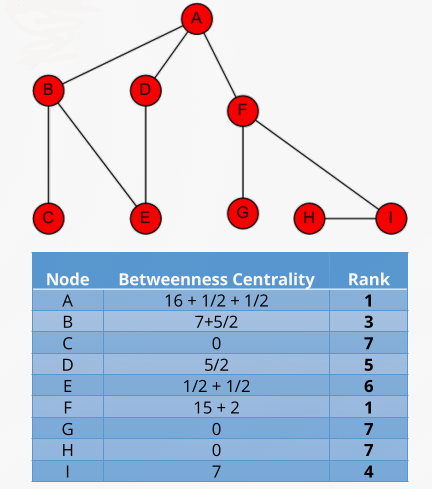
\includegraphics[width=0.4\linewidth]{figures/bet_cen.png}
      \end{figure}
    \subsubsection{Betweenness centrality normalizzata}
      Nel caso migliore il nodo $v_i$ è su tutti gli shortest paths da $s$ a $t$, quindi $\frac{\sigma_{st}(v_i)}{\sigma_{st}}=1,\forall s,t$
      $$C_b(v_i)=\sum_{s\neq t\neq v_i}\frac{\sigma_{st}(v_i)}{\sigma_{st}}=\sum_{s\neq t\neq v_i}1=2\binom{n-1}{2} = (n-1)(n-2)$$
      Quindi il valore massimo è $(n-1)(n-2)$, per normalizzarlo:
      $C^{norm}_b(v_i)=\frac{C_b(v_i)}{2(\binom{n-1}{2})}$
    \subsubsection{Centralità di vicinanza (Closeness centrality)}
      $$C_c(v_i)=\frac{1}{\bar{l}_{v_i}}$$
      I nodi influenti / centrali possono raggiungere velocemente gli altri nodi (considero gli shortest path verso tutti gli altri nodi).
      $$\bar{l}_{v_i}=\frac{1}{n-1}\sum_{v_j\neq v_i}l_{i,j}$$
      \begin{itemize}
        \item $l_{i,j}$: lunghezza cammino più breve da $v_i$ a $v_j$;
        \item $\bar{l}_{v_i}$: lunghezza media dei cammini più brevi più brevi da $v_i$.
      \end{itemize}
      \begin{figure}[H]
          \centering
          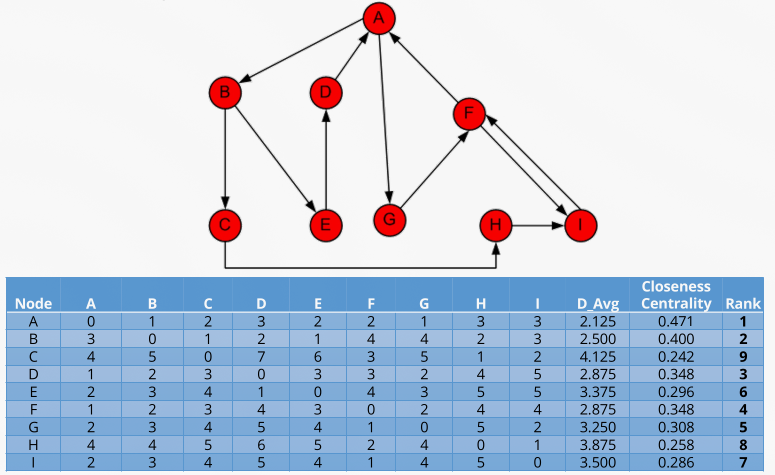
\includegraphics[width=0.5\linewidth]{figures/cl_cen.png}
      \end{figure}
    \subsubsection{Confronti}
      \begin{figure}[H]
          \centering
          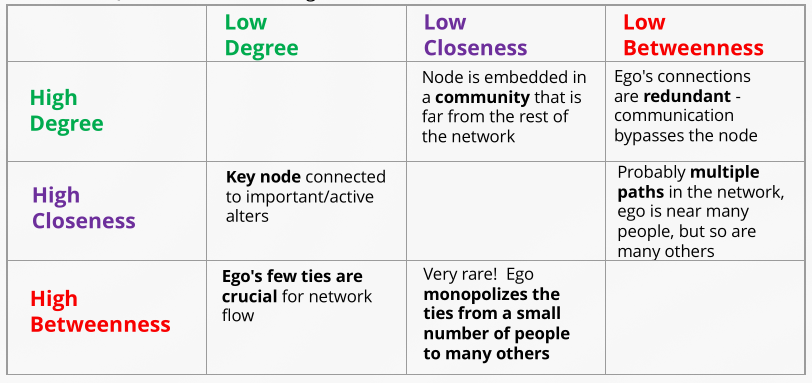
\includegraphics[width=0.6\linewidth]{figures/centr_chart.png}
      \end{figure}
  \subsection{PageRank}
    Archi che vengono da \textbf{nodi importanti} (più centrali) dovrebbero \textbf{aumentare di più la centralità} rispetto a archi che vengono da nodi meno centrali.
    \begin{figure}[H]
        \centering
        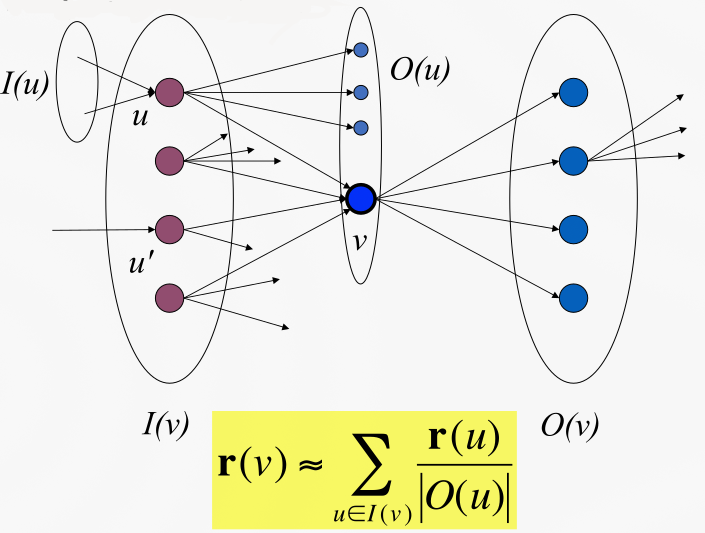
\includegraphics[width=0.3\linewidth]{figures/p_rank.png}
    \end{figure}
    Notazione:
    \begin{itemize}
        \item $r(v)$ PageRank della pagina $v$;
        \item $I(v)$ set di paine che citano $v$;
        \item $O(v)$ set di pagine citate da $v$.
    \end{itemize}
    Ogni pagina $u$ ha il suo valore PageRank $r(u)$, la pagina $v$ riceve dalla pagina $u$ una porzione del suo PageRank uguale alla porzione ricevuta da tutte le altre pagine citate da $u$: $\frac{r(u)}{\abs{O(u)}}$
    \subsubsection{PageRank - vettori e matrici}
      Si possono collezionare tutti i valori PageRank di tutte le pagine $u_i$ in un vettore $r=[r(u_0), r(u_1), ..., r(u_n)$ 
      \\
      \noindent
        \begin{minipage}[t]{0.48\linewidth}
          Si costruiscono i vettori $r$ \textbf{iterativamente, tutti assieme}. Per andare da $r_0$ iniziale a $r_1$ mediante una matrice \textbf{P} tale che $r_{i+1}=r_i\times P$.
        \end{minipage}
        \hfill
        \begin{minipage}[c]{0.48\linewidth}
            \centering
            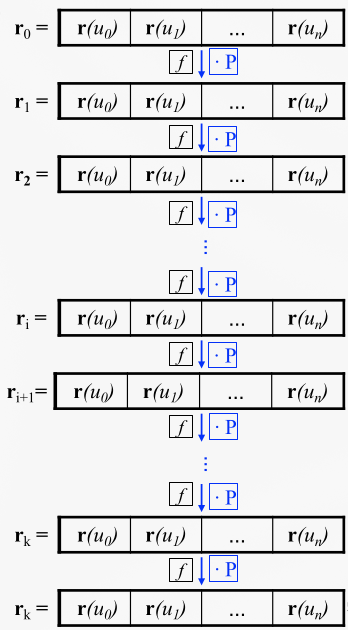
\includegraphics[width=0.5\linewidth]{figures/p_rank_m.png}
        \end{minipage}
    \subsubsection{Markov chain}
      Dato un grafo / matrice di adiacenza con $n$ stati si ha una matrice $n\times n$ P con le probabilità di transizione. A ciascun istante di tempo la catena di Markov è in uno degli $n$ stati.
      \\
      $\forall$ stato corrente $i\in [1..n]$, la catena di Markov (\textbf{P}) dice la probabilità che il prossimo stato sia $j$, $\forall j\in [1..n]$.
      \begin{figure}[H]
          \centering
          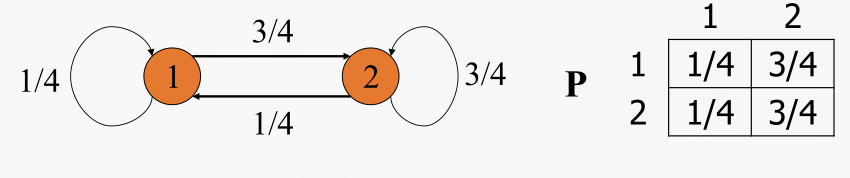
\includegraphics[width=0.7\linewidth]{figures/mar_ch.png}
      \end{figure}
      Si può rappresentare la posizione corrente in uno stato $i$ con un vettore $x=(x_1,...,x_n)$ dove tutti i componenti hanno valore 0 tranne l'$i$-esimo che ha valore 1 e rappresenta la posizione nello stato $i$.
      \\
      Il vettore di probabilità nel prossimo step si può trovare guardando la matrice P alla $i$-esima riga, in modo da controllare le probabilità per procedere al prossimo stato partendo da $i$.
    \subsubsection{Markov chain - autovettore}
      Quindi, per ogni step $x_{i+1}=x_i\times P$ ma stiamo cercando una distribuzione stabile $x_{i+1}=x_i$, cerchiamo quindi $x$ tale che $x=x\times P$ ($x$ autovettore di $P$).
      \\
      Per ogni catena \textbf{ergodica} (\textbf{fortemente connessa} e in cui in ogni step si può \textbf{essere in ogni stato} con probabilità $>$ 0) ogni stato ha un rate di visite a lungo termine per cui viene visitato proporzionalmente.
    \subsubsection{Teleporting}
      Nella pratica (Web) non sempre si hanno situazioni ergodiche, ma navigando si potrebbe "saltare" ad un'altra pagina random: "ciascuna pagina è collegata con qualsiasi altra pagina" (con basse probabilità).
      \begin{figure}[H]
          \centering
          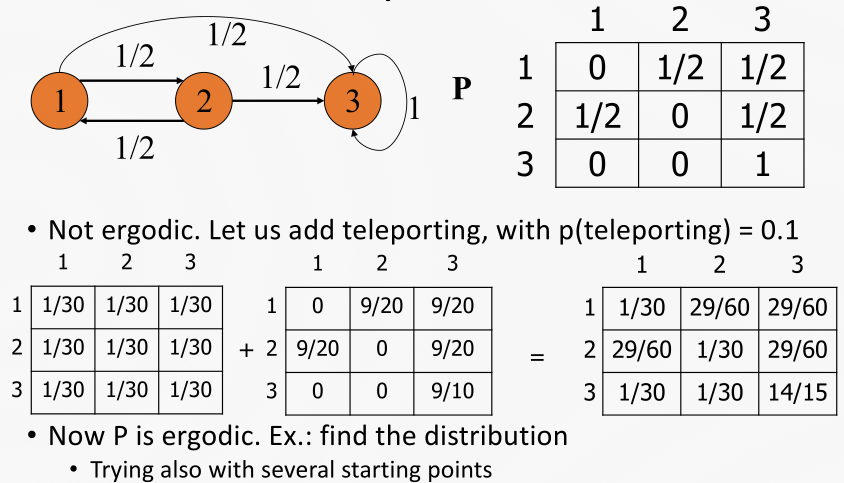
\includegraphics[width=0.6\linewidth]{figures/telep.png}
      \end{figure}
    \subsubsection{PageRank - implementazione}
      Catena di Markov, ogni pagina ha una propria probabilità per cui, durante il percorso random tra le pagine, l'utente si trovi lì
      \begin{figure}[H]
          \centering
          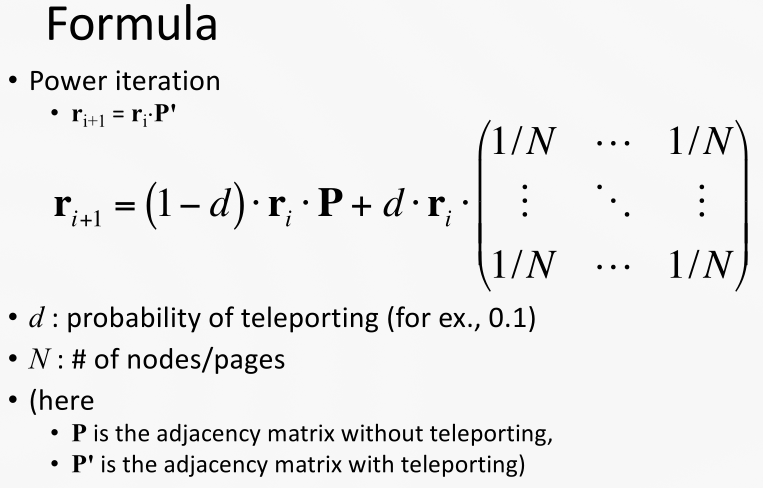
\includegraphics[width=0.4\linewidth]{figures/pr_impl.png}
      \end{figure}
      \begin{enumerate}
          \item Costruzione matrice $P'$ (matrice di adiacenza $P$ + teleporting (ergodic));
          \item Inizio da vettore di probabilità $r_0$;
          \item $r_{i+1}=r_i\times P$;
          \item Se $\abs{r_{i+1}-r_i} < \epsilon$ stoppa, altrimenti ripeti;
          \item Il vettore $r$ trovato ($r=r\times P'$, o $r~r\times P'$) è il PageRank di tutte le pagine, e ~ l'autovettore di $P'$.
      \end{enumerate}
  \subsection{HITS}
    Idea: costruire 2 set di pagine collegati:
    \begin{itemize}
        \item \textbf{Hub pages (H)} contenenti (buoni) link ad altre pagine (yahoo, buoni bookmark,...);
        \item \textbf{Authority pages (A)} con persone / entità ben organizzate nel web (w3c, Knuth's homepage,...).
    \end{itemize}
    L'algorito lavora su un set ristretto di pagine Root Set (\textit{RS}), che si espande con:
    \begin{itemize}
        \item $I(v)$ in-pages (tutte le pagine $u$ tali che $\exists v\in RS,  u \rightarrow v$);
        \item $O(v)$ out-pages (tutte le pagine $u$ tali che $\exists v\in RS,  v \rightarrow u$).
    \end{itemize}
    Si ottiene così il Base Set (\textit{BS}) con buone pagine candidate Hub / Authority e su cui l'algoritmo poi lavora, selezionando H e A mediante un controllo su ogni pagina $x$ in \textit{BS} per i valodi di \textbf{hubness} ($h(x)$) e \textbf{authority} ($a(x)$).
    \begin{figure}[H]
        \centering
        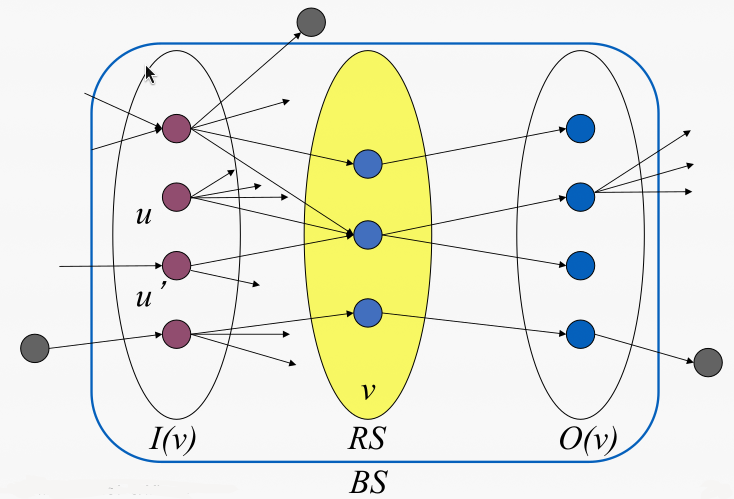
\includegraphics[width=0.3\linewidth]{figures/rs_bs.png}
    \end{figure}
    \begin{figure}[H]
        \centering
        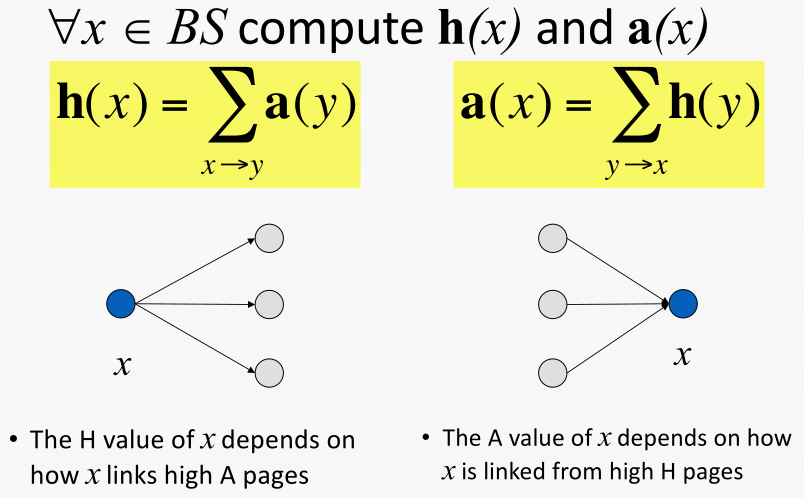
\includegraphics[width=0.3\linewidth]{figures/rs_bs_ap.png}
    \end{figure}
    \subsubsection{Procedimento - "Algoritmo"}
      \begin{enumerate}
          \item Assegnazione valori iniziali di $h(x)$ e $a(x)$ a ogni pagina $x$ del $BS$ (inizialmente $h(x)=a(x)=1$);
          \item Aggiornamento iterativo, con la precedente formula, di $h(x)$ e $a(x)$;
          \item Stop quando converge ($h(x)$ e $a(x)$ non variano più);
          \item Alla fine si riconoscono pagine "top hub" e "top authority".
      \end{enumerate}
    \subsubsection{HITS - vettori e matrici}
      Formalizzazione in vettori / matrici come PageRank.
      \begin{figure}[H]
          \centering
          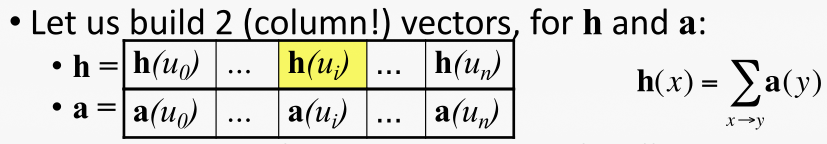
\includegraphics[width=0.7\linewidth]{figures/hits_v_m.png}
      \end{figure}
      Per calcolare $h$ dell'i-esimo componente si sommano tutti i componenti corrispondenti alle out-pages di $u_i$ e si sommano, moltiplicando quindi $a$ per \textit{l'i-esima riga della matrice di adiacenza}.
      \begin{figure}[H]
          \centering
          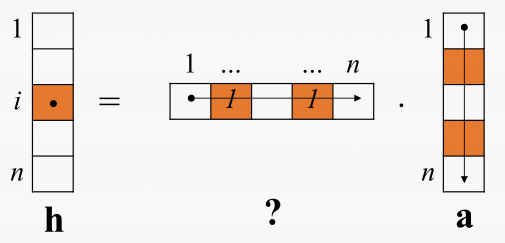
\includegraphics[width=0.3\linewidth]{figures/hits_v_m_mol.png}
      \end{figure}
      Quindi, moltiplicando l'i-esima riga di $M$ per $a$ si ottiene l'i-esimo componente di $h$, e moltiplicando tutta $M$ per $a$ si ottiene tutto $h$.
      $$h=Ma$$
      e, di conseguenza:
      $$a=M^Th$$
    \subsubsection{HITS - autovettori}
      Se abbiamo
      \begin{itemize}
          \item $h=Ma$
          \item $a=M^Th$
      \end{itemize}
      per sostituzione otteniamo
      \begin{itemize}
          \item $h=Ma=MM^Th$
          \item $a=M^Th=M^TMa$
      \end{itemize}
      $h$ è quindi l'autovettore di $MM^T$ e $a$ è l'autovettore di $M^TM$.
    \subsubsection{HITS - \texorpdfstring{$MM^T$}{MM\textasciicircum T}}
      \begin{figure}[H]
          \centering
          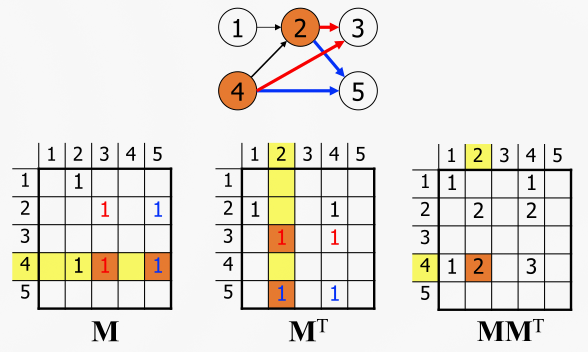
\includegraphics[width=0.5\linewidth]{figures/mmt.png}
      \end{figure}
      Questa matrice rappresenta l'\textbf{Accoppiamento Bibliografico} (Bibliographic Coupling). Ci dice quanto due nodi sono simili basandosi su "chi citano" (o chi linkano).
      \begin{itemize}
          \item \textbf{Definizione:} Il valore nella cella $\mathbf{MM}^T[i,j]$ conta il numero di nodi che sono \textbf{co-linkati} da $i$ e da $j$. In altre parole, conta quante destinazioni hanno in comune.
          \item \textbf{La Logica Matematica:}
            Il valore aumenta di 1 quando esiste un nodo $k$ che funge da "ponte comune", tale che:
            $$\mathbf{M}[i,k] = 1 \quad \text{e} \quad \mathbf{M}[j,k] = 1 $$
            \textit{(Ovvero: $i$ linka $k$ E $j$ linka $k$).}
          \item \textbf{Esempio (dalla figura):}
            Consideriamo $\mathbf{MM}^T[4,2]$ (incrocio tra nodo 4 e nodo 2). Il risultato è \textbf{2}.
            \begin{itemize}
                \item Il nodo 4 punta verso: 2, \textbf{3}, \textbf{5}.
                \item Il nodo 2 punta verso: \textbf{3}, \textbf{5}.
                \item Hanno in comune i nodi \textbf{3} e \textbf{5} $\rightarrow$ Totale: 2 destinazioni comuni.
            \end{itemize}
          \item \textbf{Proprietà:}
            \begin{itemize}
                \item La matrice è sempre \textbf{simmetrica} ($\mathbf{MM}^T[i,j] = \mathbf{MM}^T[j,i]$).
                \item Sulla diagonale principale ($\mathbf{MM}^T[i,i]$) troviamo il grado di uscita (out-degree) del nodo $i$, cioè quanti link totali partono da quel nodo.
            \end{itemize}
      \end{itemize}
    \subsubsection{HITS - \texorpdfstring{$M^T M$}{M\textasciicircum T M}}
      \begin{figure}[H]
          \centering
          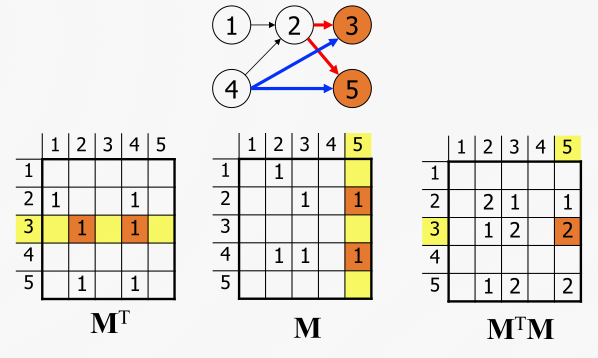
\includegraphics[width=0.5\linewidth]{figures/mtm.png}
      \end{figure}
      Questa matrice rappresenta la \textbf{Co-citazione} (Co-citation). È il concetto duale rispetto al precedente: misura la similarità tra due nodi basandosi su "chi li linka" (chi punta a loro).
      \begin{itemize}
          \item \textbf{Definizione:} Il valore nella cella $\mathbf{M}^T\mathbf{M}[i,j]$ conta quanti nodi esterni puntano SIA al nodo $i$ CHE al nodo $j$.
          \item \textbf{La Logica Matematica:}
            Il valore aumenta di 1 quando esiste un nodo $k$ (una fonte comune) tale che:
            $$\mathbf{M}[k,i] = 1 \quad \text{e} \quad \mathbf{M}[k,j] = 1 $$
            \textit{(Ovvero: $k$ linka $i$ E $k$ linka $j$).}
          \item \textbf{Esempio (dalla figura):}
            Consideriamo $\mathbf{M}^T\mathbf{M}[3,5]$ (incrocio tra nodo 3 e nodo 5). Il risultato è \textbf{2}.
            \begin{itemize}
                \item Chi punta al nodo 3? I nodi \textbf{2} e \textbf{4}.
                \item Chi punta al nodo 5? I nodi \textbf{2} e \textbf{4}.
                \item I "citanti" in comune sono il \textbf{2} e il \textbf{4} $\rightarrow$ Totale: 2 fonti comuni.
            \end{itemize}
          \item \textbf{Proprietà:}
            \begin{itemize}
                \item Anche questa matrice è sempre \textbf{simmetrica} ($\mathbf{M}^T\mathbf{M}[i,j] = \mathbf{M}^T\mathbf{M}[j,i]$).
                \item Sulla diagonale principale ($\mathbf{M}^T\mathbf{M}[i,i]$) troviamo il \textbf{grado di ingresso} (in-degree) del nodo $i$, cioè quanti link totali arrivano a quel nodo.
            \end{itemize}
      \end{itemize}
      \begin{figure}[H]
          \centering
          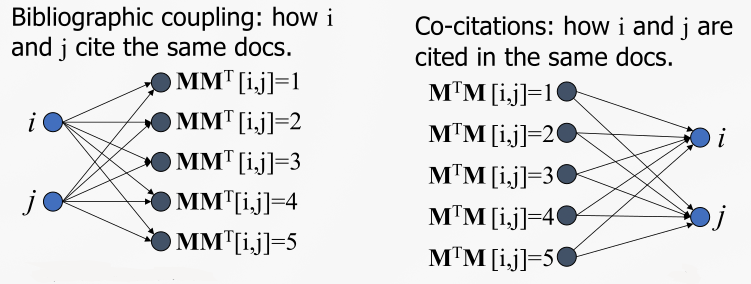
\includegraphics[width=0.8\linewidth]{figures/aut_conf.png}
      \end{figure}
  \subsection{PageRank / HITS - confronto}
    \begin{itemize}
        \item \textbf{PageRank} (Google)
          \begin{itemize}
              \item \textbf{PRO:} Robusto contro lo spam (è difficile farsi linkare da siti autorevoli), indice di qualità valido per l'intero Web.
              \item \textbf{CONTRO:} Non è specifico per la query (è un valore statico calcolato "offline"), calcolo complesso su grafi immensi.
          \end{itemize} 
        \item \textbf{HITS} (Kleinberg)
          \begin{itemize}
              \item \textbf{PRO:} Specifico per la query (viene calcolato sul sottografo dei risultati), distingue tra \textit{Hubs} e \textit{Authorities}.
              \item \textbf{CONTRO:} Facilmente spammabile (basta creare falsi Hub), problemi di convergenza, costo computazionale alto.
          \end{itemize}
    \end{itemize}
\section{Social Network Analysis - termnologia}
  \begin{figure}[H]
      \centering
      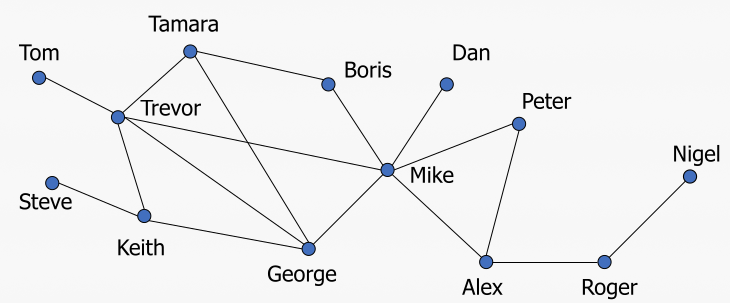
\includegraphics[width=0.6\linewidth]{figures/sna_term.png}
  \end{figure}
  \begin{itemize}
      \item \textbf{Local bridge}: arco tra due nodi ce sarebbero altrimenti "lontani", ha un \textbf{grado k} (NON IL GRADO DEL NODO) che rappresenta la distanza che ci sarebbe senza quell'arco (Tamara - Boris ha grado 3);
      \item \textbf{Global bridge}: arco che, se rimosso, disconnetterebbe la rete (Trevor - Tom, Alex - Roger);
      \item \textbf{Triangle}: sottografo completo di 3 nodi (Trevor - George - Keith);
      \item \textbf{Weak tie}: arco che appartiene a qualche triangolo (Mike - Peter);
      \item \textbf{Strong tie}: arco che appartiene a molti triangoli (Trevor - George);
      \item \textbf{Geodensic} (tra due nodi): cammino più corto tra di loro, distanza = n° archi (geodensico tra Tom e Mike = Tom - Trevor - Mike);
      \item \textbf{Diametro} di una rete: geodensico più lungo della rete (Steve - Niegel: 6);
      \item \textbf{Grado} di un nodo: n° di archi (differenzia in in-degree e out-degree su reti con direzioni);
      \item \textbf{Distribuzione di grado}: per ogni grado, il numero di nodi aventi quel grado;
      \item \textbf{Densità}: proporzione di archi che ha la rete (n° archi / n° massimo possibile nella rete);
      \item \textbf{Coefficiente di clustering} (C) di un nodo: n° archi con i suoi vicini / n° massimo possibile con i vicini ($n(n-1)/2$) ($C(Keith)=1/(3*2/2)=1/3$), il \textbf{C} della rete è pari alla media su tutti i nodi.  
  \end{itemize}
  \begin{figure}[H]
      \centering
      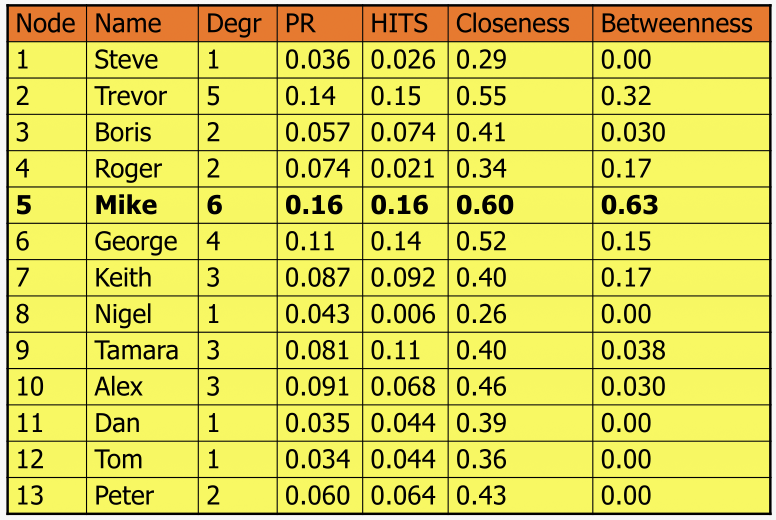
\includegraphics[width=0.5\linewidth]{figures/sna_ex.png}
  \end{figure}
  \noindent
    \begin{minipage}[c]{0.48\linewidth}
        \centering
        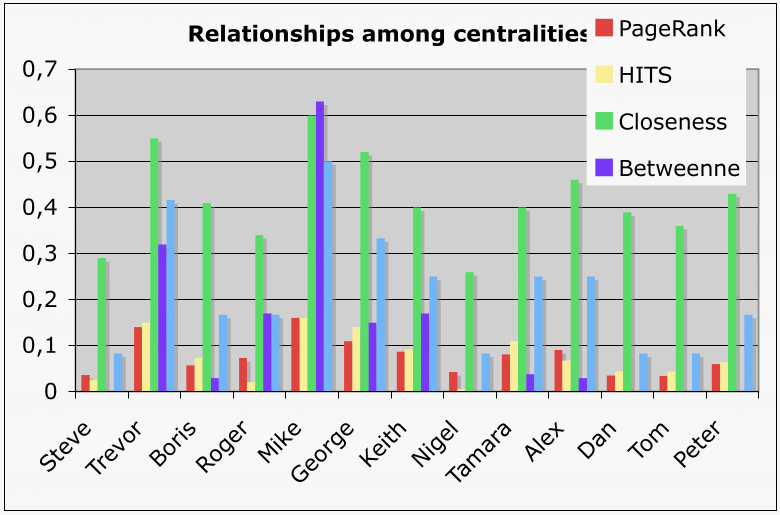
\includegraphics[width=\linewidth]{figures/sna_ex2.png}
    \end{minipage}
    \hfill
    \begin{minipage}[c]{0.48\linewidth}
        \centering
        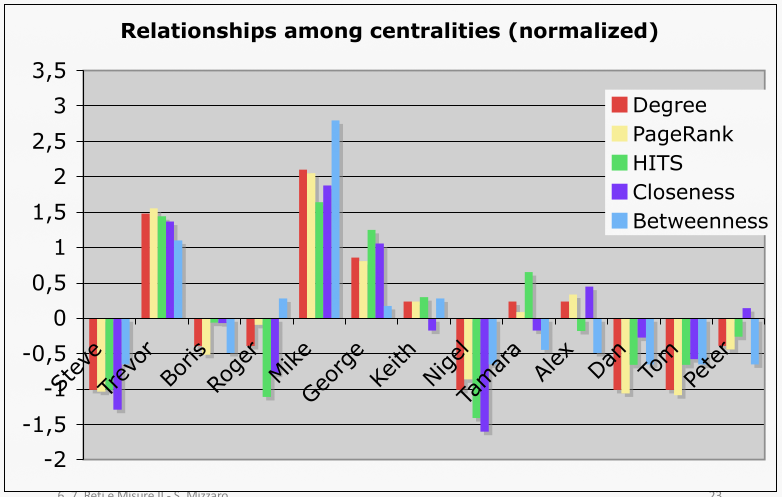
\includegraphics[width=\linewidth]{figures/sna_ex3.png}
    \end{minipage}
\section{Transitività}
  In una rete sociale si ha \textbf{transitività} quando "un amico di un mio amico è mio amico", ha come indici \textit{coefficiente di clustering locale} (relativo a singolo punto) e \textit{coefficiente di clustering globale} (relativo alla rete, media deli altri), questi sono correlati ma $\neq$.
  \subsection{Coefficiente di clustering locale}
    Misura la transitività a livello dei singoli nodi, controllando quanto i vicini di un nodo $v_i$ sono a loro volta connessi.
    \begin{figure}[H]
        \centering
        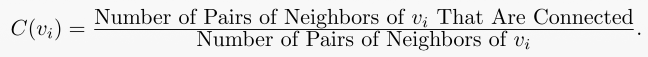
\includegraphics[width=0.8\linewidth]{figures/clustering_locale.png}
    \end{figure}
    In un grafo indiretto il denominatore è $\binom{d_i}{2}=d_i(d_i-1)/2$.
    \begin{figure}[H]
        \centering
        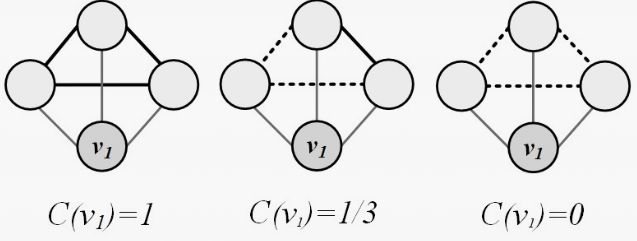
\includegraphics[width=0.5\linewidth]{figures/clustering_locale_es.png}
    \end{figure}
    \begin{itemize}
        \item Linee sottili: connessioni ai vicini;
        \item Linee trattegiate: archi mancanti fra vicini;
        \item Linee spesse: vicini connessi (quando nessun vicino è connesso $C=0$, quando tutti sono connessi $C=1$).
    \end{itemize}
  \subsection{Coefficiente di clustering globale}
    Misura transitività in grafi indiretti in 3 modi equivalenti:
    \begin{figure}[H]
        \centering
        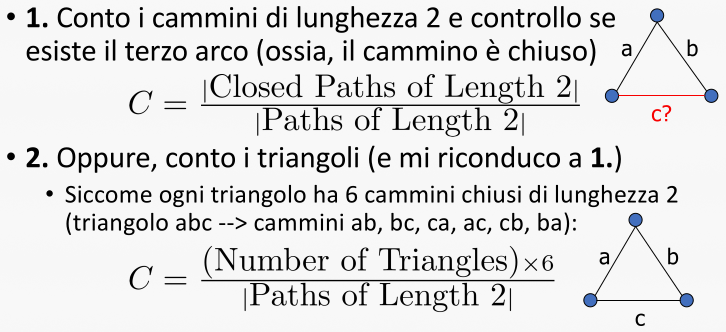
\includegraphics[width=0.6\linewidth]{figures/clustering_glob_1.png}
    \end{figure}
    \begin{figure}[H]
        \centering
        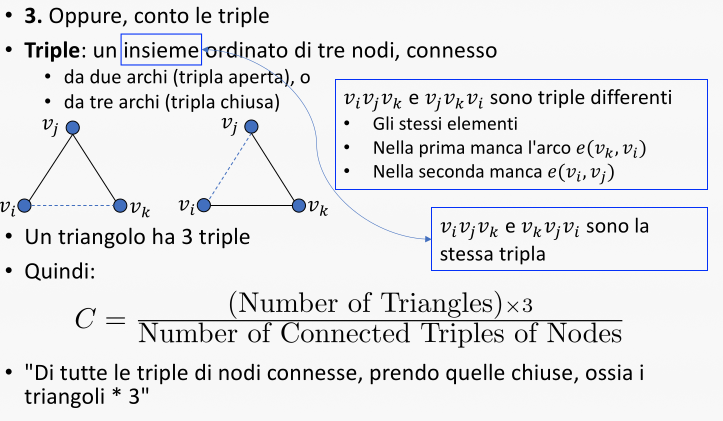
\includegraphics[width=0.6\linewidth]{figures/clustering_glob_2.png}
    \end{figure}
    \begin{figure}[H]
        \centering
        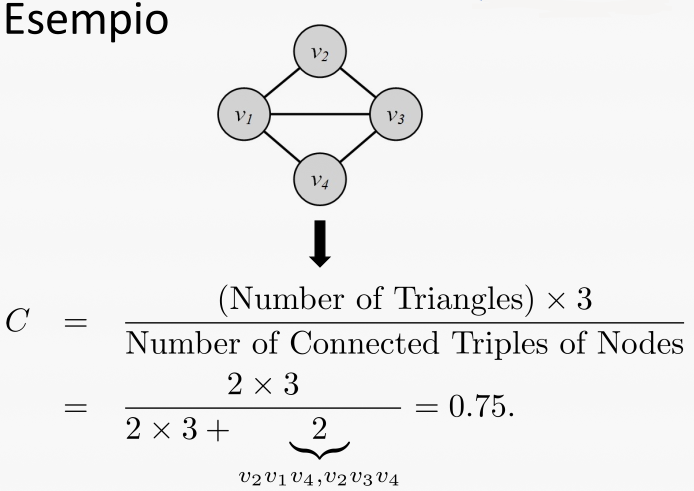
\includegraphics[width=0.6\linewidth]{figures/clustering_glob_es.png}
    \end{figure}
\section{Reciprocità}
  "Se tu mi diventi amico, anche io divento amico tuo", se nodo $v$ è connesso a nodo $u$, $u$ connettendosi a $v$ manifesta reciprocità.
  \subsection{Calcolo}
    Conto numero di \textbf{coppie reciproche} nel grafo:
    \begin{itemize}
        \item Uso matrice di adiacenza $A$;
        \item La sommatoria aggiunge 1 per ogni coppia reciproca ($A_{i,j}=A_{j,i}=1$);
        \item Divido per il numero massimo possibile di coppie reciproche dati gli archi in $E$: $\abs{E}/2$.
    \end{itemize}
    $$R=\frac{\sum_{i,j,i<j}A_{i,j}A_{j,i}}{\abs{E}/2}=\frac{2}{\abs{E}}\sum_{i,j,i<j}A_{i,j}A_{j,i}=\frac{2}{\abs{E}}\times \frac{1}{2}Tr(A^2)=\frac{1}{\abs{E}Tr(A^2)}=\frac{1}{m}Tr(A^2)$$
    $$Tr(A)=A_{1,1}+A_{2,2}+...+A_{n,n}=\sum_{i=1}^nA_{i,i}$$
    \begin{figure}[H]
        \centering
        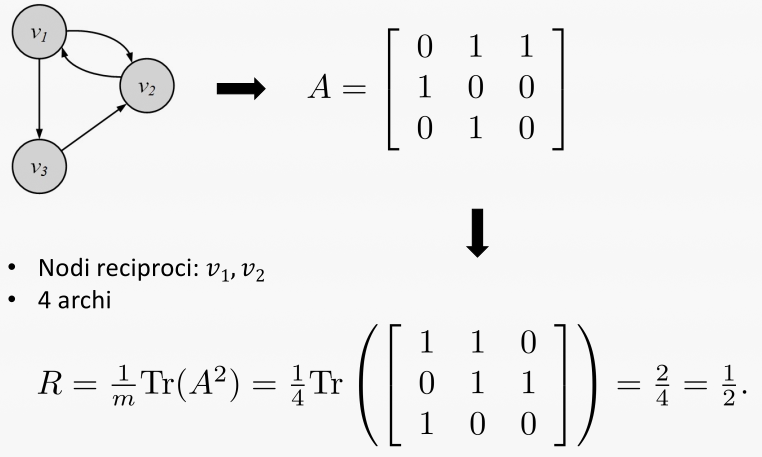
\includegraphics[width=0.6\linewidth]{figures/rec_ex.png}
    \end{figure}
\section{Bilanciamento}
  \subsection{Bilanciamento Sociale}
    Modella la \textbf{coerenza} nelle relazioni amico / nemico, formalmente si ha bilanciamento quando:
    \begin{itemize}
        \item amico di amico è amico;
        \item amico di nemico è nemico;
        \item nemico di nemico è amico;
        \item nemico di amico è nemico.
    \end{itemize}
    Si modella con reti / grafi di \textbf{'+'} e \textbf{'-'} (signed graph), in cui archi positivi hanno valore +1 e archi negativi hanno valore -1. Un triangolo di nodi $i,j,k$ è bilanciato se $w_{ij}w_{jk}w_{ki}\ge 0$
    \begin{figure}[H]
        \centering
        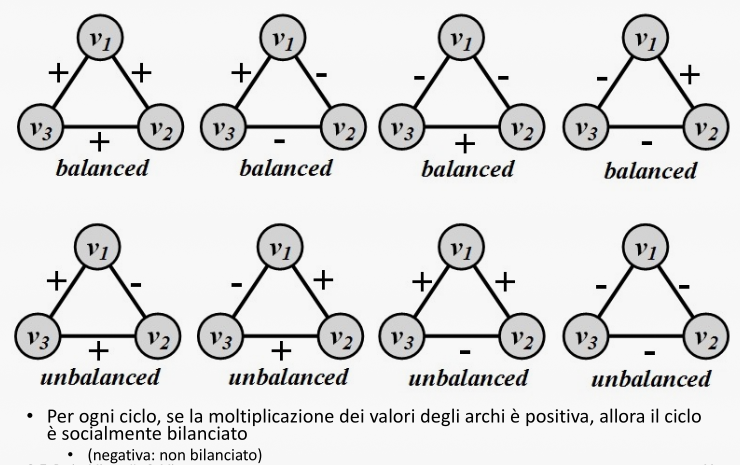
\includegraphics[width=0.6\linewidth]{figures/bilanc_es.png}
    \end{figure}
  \subsection{Status sociale}
    Quando un indivuduo è prestigioso all'interno della società: se $X$ ha status più alto di $Y$ e $Y$ più alto di $Z$ allora $X$ dovrebbe avere status più alto di $Z$... questi \textbf{cicli} sono problematici.
    \begin{figure}[H]
        \centering
        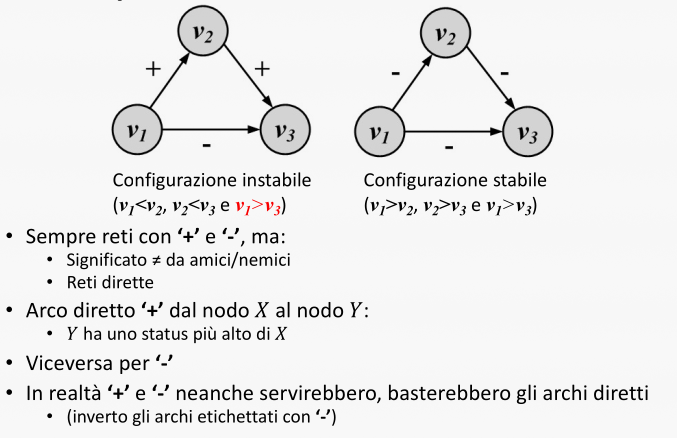
\includegraphics[width=0.5\linewidth]{figures/status_es.png}
    \end{figure}
\section{Degree distributions reali}
  \begin{itemize}
      \item Popolarità siti web:
        \begin{itemize}
            \item Tanti siti sono visitati < 1000 volte / mese (poco popolari);
            \item Pochi siti sono visitati > 1M volte / giorno (molto popolari).
        \end{itemize}
      \item Attività utenti:
        \begin{itemize}
            \item Utenti di SM sono spesso attivi su pochi siti;
            \item Alcuni (pochi) individui sono attivi su tanti siti.
        \end{itemize}
      \item Prezzi dei prodotti:
        \begin{itemize}
            \item Tantissimi prodotti a prezzo basso;
            \item Pochi prodotti costosi.
        \end{itemize}
      \item Amicizia:
        \begin{itemize}
            \item Tanti individui con pochi amici;
            \item Pochi individui con migliaia di amici.
        \end{itemize}
      \item Distribuzioni dei gradi:
        \begin{itemize}
            \item Tanti nodi con grado basso;
            \item Pochi nodi con grado alto.
        \end{itemize}
  \end{itemize}
\section{La Legge di Potenza (Power Law)}
  \subsection{Che cos'è (In parole povere)}
    La \textbf{Power Law} è una relazione matematica che descrive fenomeni dove eventi "piccoli" sono comunissimi, mentre eventi "giganti" sono rari ma esistono.
    \begin{itemize}
        \item \textbf{Formula base:} $f(k) \sim \frac{1}{k^\alpha}$
        \item \textbf{Significato:} La frequenza decresce molto velocemente man mano che cresce la grandezza ($k$).
        \item \textbf{Esempio intuitivo:} Pensa ai follower su Instagram.
        \begin{itemize}
            \item Miliardi di persone hanno pochi follower (la "coda" lunga del grafico).
            \item Pochissimi influencer (la "testa") ne hanno milioni.
        \end{itemize}
    \end{itemize}
  \subsection{Il trucco del Grafico Log-Log}
    Se disegni una Power Law su un grafico normale, ottieni un'\textbf{iperbole} (una curva a forma di "L") difficile da analizzare.
    Per capire se una rete segue davvero questa legge, si usa la scala logaritmica su entrambi gli assi.
    \begin{itemize}
        \item \textbf{La Magia:} Se applichi il logaritmo alla formula $f(k) = C/k^\alpha$, trasformi le moltiplicazioni in addizioni:
          $$ \log(f(k)) = \log(C) - \alpha \log(k) $$
        \item \textbf{Risultato:} Questa è l'equazione di una \textbf{retta} ($y = q - mx$).
        \item \textbf{Regola d'oro:} Se metti i dati su un grafico log-log e vedi una linea dritta che scende, allora sei davanti a una Power Law. La pendenza della retta è l'esponente $\alpha$.
    \end{itemize}
  \subsection{Esempi Reali (Dalle Slide)}
    \begin{itemize}
        \item \textbf{Telefonate ($1/k^2$):} Pochissimi numeri ricevono milioni di chiamate, la maggioranza ne riceve poche.
        \item \textbf{Libri ($1/k^3$):} Pochi best-seller vendono milioni di copie, la maggioranza dei libri vende quasi zero.
        \item \textbf{Citazioni Scientifiche ($1/k^3$):} Pochi paper (tipo quelli di Einstein) sono citati da tutti, la maggior parte dei paper non li legge nessuno.
        \item \textbf{Social Network ($1/k^2$):} La distribuzione dei follower (in-degree).
    \end{itemize}
  \subsection{Nota: Differenza con Zipf}
    \begin{itemize}
        \item \textbf{Power Law:} Sull'asse X metti il \textbf{valore} (es. "Quanti hanno 100 amici?").
        \item \textbf{Zipf:} Sull'asse X metti la \textbf{classifica/rank} (es. "Chi è il 1°, il 2°, il 3° più ricco?").
    \end{itemize}
  \subsection{Test}
    Per capire se rete ha degree distribution power law:
    \begin{enumerate}
        \item Calcolare grado $k$ di ogni nodo;
        \item Calcolare $p_k$, la frazione di nodi con grado $k$;
        \item Disegnare grafico su scala log-log con $k$ su asse X e $p_k$ su asse Y;
        \item Se è power law, linea retta.
    \end{enumerate}
    NON è un approccio sistematico! Altre distribuzioni potrebbero avere lo stesso pattern.
  \subsection{Coefficiente di clustering}
    Nelle reti sociali reali connessioni sono \textbf{molto transitive} (amici di un utente sono amici tra di loro, dormando \textbf{triangoli} con alto clustering).
\section{Diffusione informazioni}
  Un rumor si diffonde su una rete sociale, tutti gli utenti lo passano immediatamente a tutti gli amici. Quanti hop servono per raggiungere tutti i nodi?
  \subsection{Milgram}
  \noindent
    \begin{minipage}[c]{0.48\linewidth}
        Partendo da 296 persone a caso (196 Nebraska / 100 Boston) gli viene chiesto di spedire una lettera via intermediari a un agente di borsa a Boston, potendo spedire solo a persone che conoscevano personalmente. Fra tutte le (64) lettere che arrivarono a destinazione il n° medio di passaggi fu circa 6.
    \end{minipage}
    \hfill
    \begin{minipage}[c]{0.48\linewidth}
        \centering
        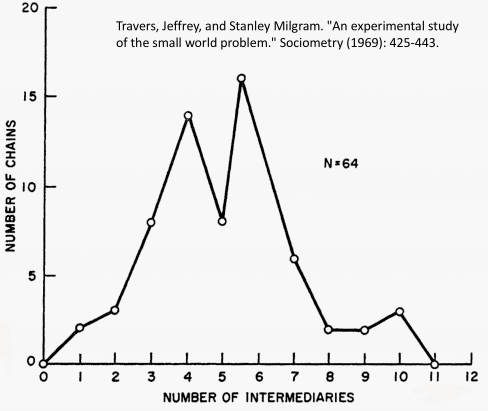
\includegraphics[width=0.8\linewidth]{figures/milgram.png}
    \end{minipage}
  \subsection{Dodds}
    Esperimento di Milgram mandato per email, confermato tasso di risposta e sei gradi di separazione.
  \subsection{Erdos}
    Ricerca n° di link per connettere uno scienziato / studioso mediante co-authorship di articoli scientifici, lunghezza dei cammini fra matematici: \textbf{media} 4.65, \textbf{massima} 13.
  \subsection{Proprietà reti reali}
    \begin{itemize}
        \item Solitamente hanno struttura core-periferia: core denso con tanti archi, nodi della periferia con archi verso il core ma non fra di loro,
        \item Paradosso degli amici: grado dei vicini di un nodo $v$ è più alto del grado di $v$.
    \end{itemize}
\section{Modelli delle reti}
  \textbf{Reti reali} sono troppo grandi per valutarle univocamente, si usano quindi processi stocastici che generano / producono grafi per poterle valutare su una scala inferiore, rendendole più controllabili / analizzabili rispetto alla visione reale.
  \subsection{Reti regolari}
    \begin{figure}[H]
        \centering
        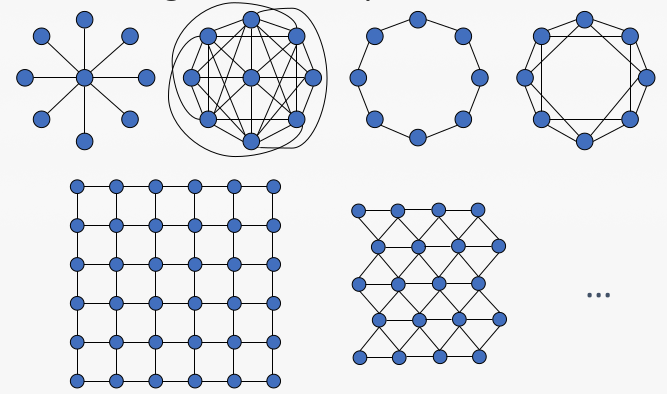
\includegraphics[width=0.5\linewidth]{figures/reti_reg.png}
    \end{figure}
    \begin{itemize}
        \item \textbf{Distanze} (Average path length / Diametro): spesso \textbf{grandi};
        \item Coefficiente di \textbf{Clustering}: spesso \textbf{alto};
        \item \textbf{Distribuzione dei gradi}: spesso con un \textbf{picco}, e spesso 0 altrove;
        \item \textbf{Connettività}: spesso \textbf{completamente connesse};
        \item Le reti al mondo raramente sono così, nemmeno quelle artificiali se grandi / complesse.
    \end{itemize}
  \subsection{Reti casuali}
    Grafo con $n$ nodi e archi casuali, studiando tutte le proprietà dei grafi e, nei grafi \textbf{grandi}, il \textbf{limite termodinamico} per $n\rightarrow \infty$. Reti interessanti se suppongo che le amicizie possano scaturire in modo casuale.
    \subsubsection{Modello G(n,m)}
      Grafo con \textbf{n nodi} fissati e \textbf{m archi} piazzati a caso fra gli $n$ nodi (solitamente indiretto, senza multi e auto archi).
      \begin{figure}[H]
          \centering
          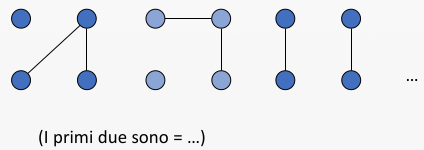
\includegraphics[width=0.6\linewidth]{figures/gnm.png}
      \end{figure}
      Si studia il caso $n\rightarrow \infty$, valutando il \textbf{caso medio}: ciò che succede in media su un insieme di tanti grafi casuali (diametro di G(n,m) = diametro medio di tutti i grafi G(n,m)). Comodo analiticamente per $n$ molto grandi, si valutano proprietà \textbf{tipiche} (più interessanti) e non casi speciali / particolari (meno interessanti).
    \subsubsection{Modello G(n,p)}
      Introdotto per determinate misure altrimenti non facilmente calcolabili, invece di fissare il \# di archi, si fissa la \textbf{probabilità p} (indipendente) \textbf{di esistenza archi}
      \begin{itemize}
        \item N° archi (medio): $<m>=\frac{n(n-1)}{2}p=\binom{n}{2}p$;
        \item Grado medio (tutte le estremità di archi / n° nodi): $<k>=\frac{2<m>}{n}=(n-1)p$, di solito denotato con $c=(n-1)p$ e approssimato con $c=np$, per $n$ grande cambia poco;
        \item \textbf{Coefficiente di Clustering}: $C=\frac{c}{n-1}$, valore molto basso ($\rightarrow 0$ per $n\rightarrow \infty$);
        \item \textbf{Diametro} (geodensica più lunga): $l=\frac{\ln n}{\ln c}$, cresce con $n$ e cala con crescere di $c$ (sorprendentmente piccolo, \textbf{small world} effect)
      \end{itemize}
      Da degree distribution e C si evince che non è un modello adeguato a modellazione reti reali.
      \begin{figure}[H]
          \centering
          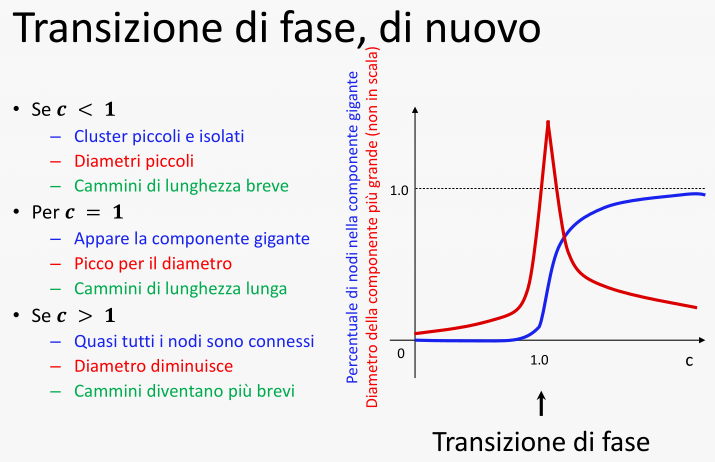
\includegraphics[width=0.6\linewidth]{figures/tran_fas.png}
      \end{figure}
    \subsubsection{Differenza}
      Si assomigliano ma $G(n,m)\neq G(n,p)$, nel primo il n° di archi è \textbf{esattamente} $m$, nell'altro è \textbf{in media} $m=p\times n(n-1)/2$.
      \begin{figure}[H]
          \centering
          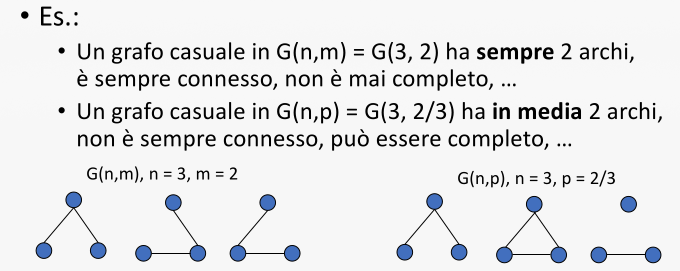
\includegraphics[width=0.6\linewidth]{figures/gnp.png}
      \end{figure}
      Entrambi hanno distribuzione dei gradi di \textbf{Poisson} / \textbf{Bernoulli} (= per $n=\infty$), non proprio simmetrica ma quasi.
    \subsubsection{G(n,p) connesso?}
      In generale no (basta un singolo nodo isolato), ma dato che $n\rightarrow \inf$, che ci sia un singolo nodo (o piccole componenti) isolato o meno non importa, basta aggiungere / togliere un arco (nodo) e si sistema. Si valuta invece esistenza "giant component", connessa e che contiene quasi tutti i nodi, e se ne valuta la dimensione:
      \begin{itemize}
          \item p = 0: grafo disconnesso - dimensione = 1 - costante a aumentare di $n$;
          \item p = 1: grafo completo - dimensione = n - aumenta con $n$.
      \end{itemize}
      \begin{figure}[H]
          \centering
          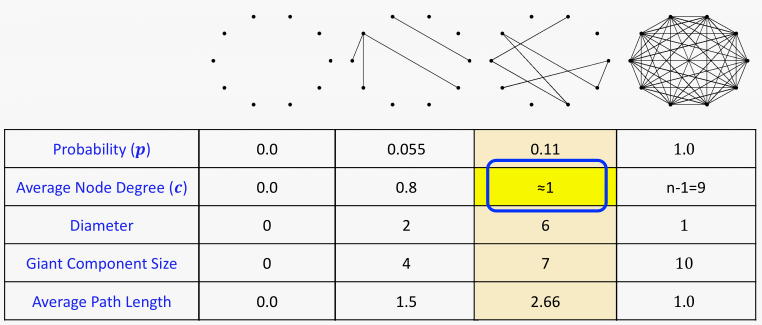
\includegraphics[width=0.6\linewidth]{figures/comp_gig.png}
      \end{figure}
      Con aumentare di p aumenterà la probabilità di avere una GC?
      \\
      Siano un grafo casuale con grado medio $c$, un insieme di nodi connesso $S$ e $S'=V-S$ l'insieme complementare (assumiamo $\abs{S}<<\abs{S'}$). Per ogni nodo $v\in S$ con un hop da $v$ visitiamo ~$c$ nodi (con un hop da un qualsiasi nodo di $S$ visito ~$\abs{S}c$ nodi). Se $S$ è piccolo, da $S\rightarrow S'$ con un hop l'insieme dei nodi connessi diventa pi grande di un fattore di $c$.
      \\
      Se è la componente connessa più grande, la sua grandezza aumenta sempre e dopo $n$ hop: $c^n\geq 1$, se invece $c<1$ il numero di nodi visitati muore.
    \subsubsection{Recap}
      Riguardo a reti reali il modello casuale:
      \begin{itemize}
          \item Modella \textbf{bene} lunghezza media dei cammini (bassa, small world);
          \item \textbf{Sottostima} drasticamente coefficiente di clustering;
          \item Non hanno distribuzione Power-law, ma \textbf{Poisson}.
      \end{itemize}
      Utile per spiegare alcuni fenomeni (small world) ma non tutti.
  \subsection{Reti small-world}
    Distanza piccola fra nodi, diametro basso e coefficiente di clustering alto.
    \subsubsection{Procedura}
      \begin{enumerate}
          \item Parto da rete regolare;
          \item Considero ogni singolo arco;
          \item Con probabilità $p$ lo ricollego casualmente (con $p$ 0 ho rete regolare, con $p$ 1 ho rete casuale).
      \end{enumerate}
    \subsubsection{Reti che ci interessano}
      Dari $n$ nodi e $c$ n° (medio) di archi per vertice ($\frac{nc}{2}$ archi totali) avremo $n\geq c\geq log(n)\geq 1$:
      \begin{itemize}
          \item Con $n\geq 1$ reti grandi con $n$ grande;
          \item Con $n\geq c$ reti sparse;
          \item Con $c\geq log(n)\geq 1$ \textit{non così sparse} da rischiare di diventare sconnesse.
      \end{itemize}
      Si valutano 2 misure:
      \begin{itemize}
          \item \textbf{L}: lunghezza media del cammino (numero di archi) minimo fra 2 nodi della rete. Misura per qunti amici devo passare per raggiungere una persona (globale);
          \item \textbf{C} coefficiente di Clustering: dato un vertice $v$ considero i suoi $k_v$ vicini e controllo quanti archi trovo fra i vicini (al massimo $k_v(k_v-1)/2$). Sia $C_v=\frac{n archi}{\frac{k_v(k_v-1)}{2}}$ la frazione degli archi effettivamente esistente, quindi \textbf{C} = media di $C_v$ su tutti i vertici della rete. Misura quanto gli amici di una persona sono amici fra di loro (locale).
      \end{itemize}
      Casi limite
      \begin{itemize}
          \item $p=0$ (regolare):
            \begin{itemize}
                \item L(0): $\frac{n}{2c} >> 1$ distanze grandi;
                \item C(0): $\frac{3}{4}$ "criccoso".
            \end{itemize}
          \item $p=1$ (random):
            \begin{itemize}
                \item L(1): $\frac{log(n)}{log(c)}$ distanze basse (small world);
                \item C(1): $\frac{c}{n} << 1$ poco "criccoso".
            \end{itemize}
      \end{itemize}
    \subsubsection{Distribuzione dei gradi}
      Distribuzione strana con picco e soglia (cutoff) inferiore $p_k=e^{-cp}\frac{(cp)^{k-c}}{(k-c)!}$.
    \subsubsection{Recap}
      Reti small-world:
      \begin{itemize}
          \item Spiegano effetto small world (non spiegato da reti regolari, "ereditato" da G(n,p));
          \item Spiega coefficiente di clustering alto (non spiegato da G(n,p), "ereditato" da reti regolari);
          \item Non spiega distribuzione dei gradi che si trova "in natura" (\textbf{no power-law}, no coda lunga, no hub).
      \end{itemize}
  \subsection{Reti scale free}
    Studio delle distribuzioni di:
    \begin{itemize}
      \item \textbf{Outdegree}: $P_{out}(k)$ probabilità che una pagina abbia $k$ outlink;
      \item \textbf{Indegree}: $P_{in}(k)$ probabilità che una pagina abbia $k$ inlink (più interessante).
    \end{itemize}
    Sono entrambe \textbf{power-law}, non poisson.
    \subsubsection{Diametro}
      Distanza \textbf{media} fra nodi (lunchezza media del cammino minimo fra 2 nodi della rete), sperimentalmente $<d>=0.35+2.06\times log(N)$ (anche aumentando molto n° nodi, diametro rimane basso $\rightarrow$ \textbf{power law} e \textbf{small-world}).
  \subsection{Reti con attaccamento preferenziale}
    \textit{Nuovo modello stocastico}, ad ogni passo aggiungo nuovo nodo e un arco che lo collega ad un nodo preesistente scelto a caso ma con probabilità non uniforme (proporzionale al \textbf{grado} del nodo esistente $P(v_i)=\frac{d_i}{\sum_jd_j}$).
    \\
    Come per gradi casuali si possono simulare reti del mondo reale generando un grafo con attaccamento preferenziale (lavorando su grafi indiretti) con un grado atteso $m$ (invece di attaccare nuovo nodo a un unico altro nodo, ne scelgo $m$).
    \begin{figure}[H]
        \centering
        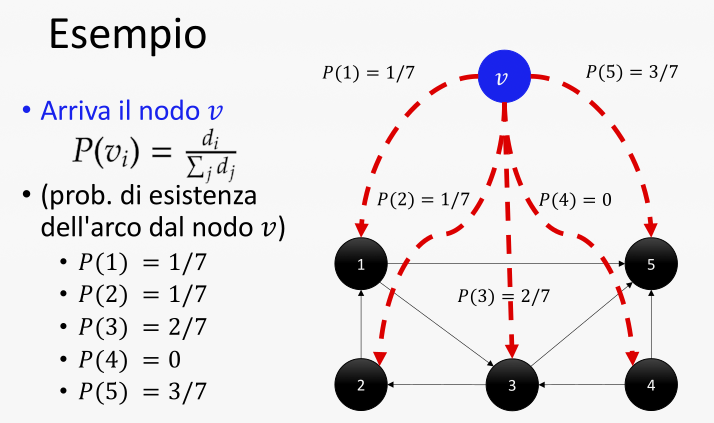
\includegraphics[width=0.5\linewidth]{figures/pref_att.png}
    \end{figure}
    \subsubsection{Sul modello scale-free}
    \textbf{Lunghezze medie} basse, ma \textbf{clustering} basso. Le scale-free hanno distribuzioni \textbf{power law}, in log-log è una retta $f(k)=\frac{C}{k^\alpha}$, ha \textbf{code lunghe} con molti nodi con $k$ basso, ci sono però pochi nodi con grado molto alto (\textbf{hub}).
  \subsection{Sunto}
    \begin{figure}[H]
        \centering
        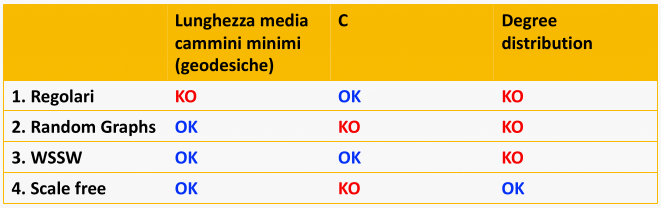
\includegraphics[width=0.6\linewidth]{figures/sunto.png}
    \end{figure}
    Insomma nessun modello "funziona", ossia crea reti uguali a quelle del mondo reale...
  \subsection{Attaccamento preferenziale non lineare}
    $$P(v_i)=\frac{d_i^\alpha}{\sum_jd_j^\alpha}$$
    \begin{itemize}
        \item Se $\alpha=1$ è l'attaccamento preferenziale originale;
        \item Se $\alpha<1$ vantaggio di avere grado alto è inferiore, no long tail, no hub;
        \item Se $\alpha>1$ vantaggio di avere grado alto è superiore, winner-takes-all (un singolo nodo connesso a tutti).
    \end{itemize}
  \subsection{Attrattività}
    $$P(v_i)=\frac{A+d_i}{\sum_j(A+d_j)}$$
    \begin{itemize}
        \item Se $A=0$ è l'attaccamento preferenziale originale;
        \item Altrimenti evita che nodi con grado 0 non ricevano link, si ottiene sempre una \textbf{power law} con pendenza che varia con $A$.
    \end{itemize}
  \subsection{Fitness}
    $$P(v_i)=\frac{\eta_id_i}{\sum_j(\eta_jd_j)}$$
    $\eta_i$ rappresenta la fitness del nodo $i$, se $\forall i,j(\eta_i=\eta_j)$ è l'attaccamento preferenziale originale, se i valori di fitness sono in un intervallo limitato: rete con + hub, si elimina dipendenza dal rich-get-richer dei nodi più vecchi, anche i nodi giovani con alta fitness competono. Si ottiene \textbf{sempre} una \textbf{power law}.
  \subsection{Random Walk}
    Parte da una piccola rete qualsiasi, ad ogni passo si aggiunge un nuovo nodo $i$, con $m>1$ archi attaccati di cui il primo è collegato con un nodo vecchio $j$ scelto a caso (probabilità \textbf{uniforme}), ogni arco degli $m-1$ restanti viene collegato:
    \begin{itemize}
        \item Con probabilità $p$ a \textbf{un vicino} di $j$ scelto a caso;
        \item Con probabilità $1-p$ a un nodo vecchio qualsiasi scelto a caso;
    \end{itemize}
    Con $p$ probabilità che si formi un triangolo.
    \begin{figure}[H]
        \centering
        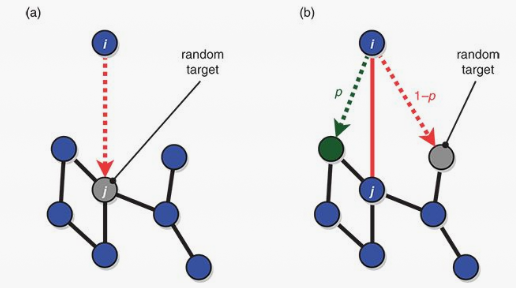
\includegraphics[width=0.4\linewidth]{figures/rand_wal.png}
    \end{figure}
    \subsubsection{FUNZIONA}
      \begin{itemize}
          \item \textbf{Degree distribution power law}: quando scelgo un vicino ($p$) tendo a scegliere nodi con grado alto (in quanto attaccamento preferenziale), si formano hub;
          \item \textbf{Cammini brevi};
          \item \textbf{Clustering alto}: presenza di triangoli.
      \end{itemize}
\section{Comunità}
  Comunità (\textbf{community}) di utenti = gruppo fornito / gestito dalla piattaforma, modellato mediante gruppo di nodi "connessi fra loro e non connessi con gli altri" (homophilia: tendenza ad associarsi con persone simili a loro).
  \begin{figure}[H]
      \centering
      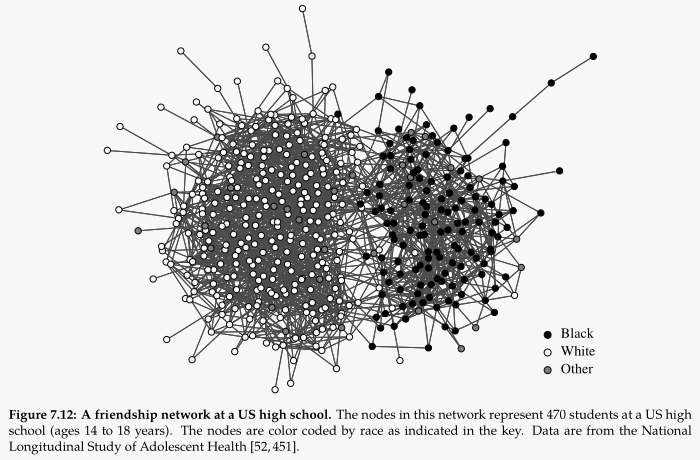
\includegraphics[width=0.5\linewidth]{figures/community_es.png}
  \end{figure}
  \subsection{Definizione "ideale"}
    Sottografo connesso e senza archi con altri nodi: dato un grafo $G$, una comunità $C$ è un sottografo di $G$ tale che $C$ è connesso (\textit{o addirittura completo}) e $\forall$ nodo $v\notin C$, $v$ è sconnesso da $C$ ($\nexists$ cammino fra $v$ e nodi di $C$).
  \subsection{Definizione "realistica"}
    Sottografo connesso e senza archi con altri nodi: dato un grafo $G$, una comunità $C$ è un sottografo di $G$ tale che $C$ è connesso e $\forall$ nodo $v\notin C$, $v$ è \textbf{poco connesso} a $C$.
  \subsection{Algoritmi per riconoscere comunità}
    \subsubsection{Edge betweenness centrality}
      \noindent
        \begin{minipage}[c]{0.48\linewidth}
            Anche gli archi possono essere più o meno centrali (si applica centralità di betweenness sugli archi), quantifica quanti shortest path passano per un arco anziché per un vertice (\textit{quanto un arco è importante nel connettere i nodi}). Gli archi con alta betweenness centrality sono i \textbf{weak ties}.
        \end{minipage}
        \hfill
        \begin{minipage}[c]{0.48\linewidth}
            \centering
            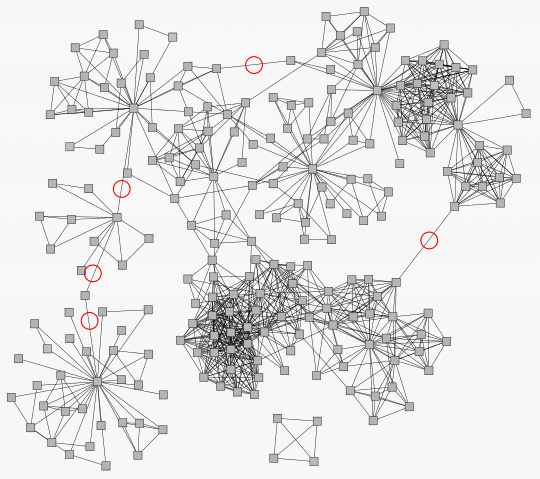
\includegraphics[width=0.8\linewidth]{figures/edge_centr.png}
        \end{minipage}
      Idea: rimuovere ricorsivamente legami deboli rimuovendo gli archi con alta betweenness centrality (\textbf{disconnettendo la rete}), rendendo le comunità componenti connesse.
    \subsubsection{Algoritmo di Givran-Newman}
      \begin{enumerate}
          \item Calcolare edge betweenness per tutti gli archi del grafo;
          \item Rimuovere arco con betweenness più alta;
          \item Ricalcolare edge betweenness per tutti gli archi del grafo (basta per quelli la cui betweenness è cambiata);
          \item Ripetere fino alla rimozione di tutti gli archi.
      \end{enumerate}
      \begin{figure}[H]
          \centering
          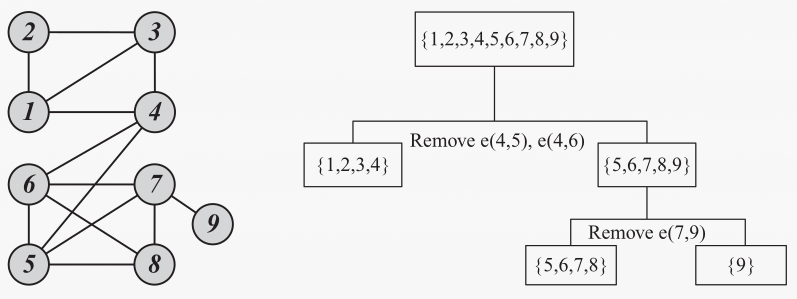
\includegraphics[width=0.7\linewidth]{figures/giv_new.png}
      \end{figure}
  \subsection{Gerarchia}
    Viene prodotto un albero (\textit{dendrogramma}) del quale ogni livello corrisponde ad un valore di edge betweenness (decrescente da radice a foglie - sopracommunità $\rightarrow$ comunità $\rightarrow$ sottocomunità).
\section{Diffuzione informazioni}
  Processo per cui un'\textbf{informazione} (video, meme), o anche \textbf{comportamento} (adozione di una tecnologia) si diffonde e raggiunge altri individui. È un fenomeno \textbf{dinamico} sulle reti, dove i player principali sono:
  \begin{itemize}
      \item \textbf{Mittente (sender)}: uno o più mittenti che iniziano il processo;
      \item \textbf{Destinatari (receivers)}: uno o più destinatari che ricevono l'informazione (insieme solitamente molto più grande di quello dei sender);
      \item \textbf{Mezzo (medium)}: mezzo tramite il quale la diffusione avviene.
      \item \textbf{Intervention}: mezzo di intervento / \textbf{intromissione} fino al blocco completo della diffusione (nel caso di fake news), al contrario possono anche "far ripartire" / velocizzare la condivisione (messaggi pubblicitari).
  \end{itemize}
  \subsection{Herd behavior}
    Network \textbf{completamente osservabile} e ho informazioni \textbf{globali}, questo comportamento descrive quando un \textbf{gruppo di individui} esegue azioni \textbf{altamente correlate} senza piani (tendenza naturale a imitare). Dev'esserci una \textbf{connessione} fra individui e un \textbf{metodo di condivisione} informazioni oppure un modo di osservare individui.
    \subsubsection{Grafo completo}
      Rappresentazione di reti herd dove nodi possono osservare almeno maggior parte degli altri nodi e possono osservare informazioni pubbliche.
    \subsubsection{Esempio}
      \begin{figure}[H]
          \centering
          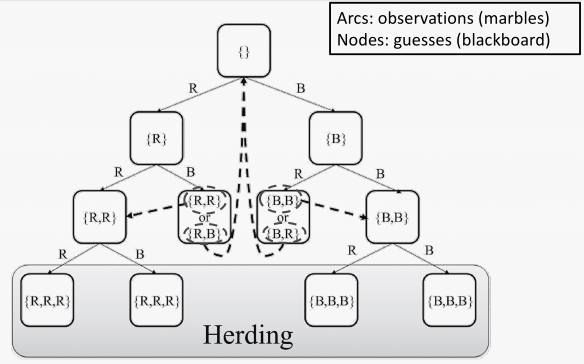
\includegraphics[width=0.4\linewidth]{figures/herding.png}
      \end{figure}
      Due possibili configurazioni (B/B/R - majority blue o R/R/B - majority red), ogni studente cerca di stimare la \textbf{conditional probability} che sia maj. blue / red data una sua estrazione e la lista delle votazioni degli altri.
      \begin{itemize}
        \item P[majority-blue] = P[majority-red] = 1/2;
        \item P[blue | majority-blue] = P[red | majority-red] = 2/3;
        \item P[blue | majority-red] = P[red | majority-blue] = 1/3.
      \end{itemize}
      \textbf{Bayes's rule}: $p(C|I)=\frac{p(C)\times p(I|C)}{p(I)}$, per cui P[majority-blue | blue] = P[blue | majority-blue] $\times$ P[majority-blue] / P[blue].
      \\
      Sapendo che P[blue] = P[blue | majority-blue] $\times$ P[majority-blue] + P[blue | majority-red] $\times$ P[majority-red] = $2/3\times1/2+1/3\times1/2=1/2$ possiamo vedere \textbf{P[majority-blue | blue]} = $(2/3\times1/2)/(1/2)=2/3>1/2$. Se le osservazioni sono \textit{blue, blue}, anche se il terzo studente osserva \textit{red} sarà portato a votare \textit{blue}.
    \subsubsection{Intervention}
      Quando una nuova \textbf{informazione privata} viene rilasciata la herd rivaluta le scelte, il che potrebbe portare a risultati completamente diversi.
  \subsection{Information cascade}
    Utenti condividono contenuti di altri utenti presenti nella rete, quindi le info si propagano tra vicini:
    \begin{itemize}
        \item individui devono essere \textbf{connessi a una rete};
        \item individui \textbf{osservano} solo \textbf{decisioni} dei \textbf{vicini immediati}.
    \end{itemize}
    La rete è un \textbf{grafo diretto} (nodi sono attori e archi appresentano canali di comunicazione tra loro), un nodo può solo influenzare nodi \textbf{a cui è connesso}. Le decisioni sono binarie (Y/N) ed i nodi possono essere \textbf{attivi} (adottano comportamento / decisione del precedente) o \textbf{inattivi} (non hanno ancora adottato). Un nodo attivo può \textbf{attivare} i nodi vicini (si può passare solo da non attivo ad attivo, non viceversa).
    \subsubsection{Independent Cascade Model (ICM)}
      Modello cascade \textbf{sender-centric} dove \textbf{ogni} nodo ha la possibilità di attivare i suoi vicini subito dopo la sua attivazione (nodi che attivano sono sender e nodi che vengono attivati sono receivers).
      \begin{itemize}
          \item Nodo attivato all'istante $t$;
          \item All'istante $t+1$ può attivare i suoi vicini;
          \item Assumiamo che $v$ sia attivato all'istante $t$:
            \begin{itemize}
              \item Per ogni vicino $w$ di $v$ c'è probabilità $p_{vw}$ che quel nodo venga attivato all'istante $t+1$;
              \item $p_{vw}$ può differire per diverse coppie di nodi.
            \end{itemize}
          \item Ogni nodo $v$ attivato all'istante $t$ ha una \textbf{singola} possibilità di attivare i suoi vicini (può solo accadere a $t+1$).
      \end{itemize}
    \subsubsection{Massimizzare spread di cascade}
      Trovare il \textbf{più piccolo} set di nodi di una rete tale il loro spread aggregato nella rete sia massimizzato: dato un \textbf{budget} $k$ si deve trovare un \textbf{initial set} $S, \abs{S}=k$ che massimizzi $f(S)$. Sappiamo che le activations sono \textbf{random}: si generano i numeri random per tutti gli archi all'inizio del processo. $f(S)$ è:
      \begin{itemize}
          \item \textbf{non negativa};
          \item \textbf{monotona} - $f(S+v)\geq f(S)$;
          \item \textbf{submodulare} - sia $N$ un set finito, un set è submodulare se e solo se:
            \begin{itemize}
                \item $f:2^N\rightarrow R$;
                \item $\forall S \subset T \subset N, \forall v\in N \setminus T$;
                \item $f(S+v)-f(S) \geq f(T+v)-f(T)$;
            \end{itemize}
            Ovvero isottoinsiemi più piccoli ci guadagnano di più.
      \end{itemize}
    \subsubsection{Problemi}
      Trovare un element set $S$ per il quale $f(S)$ è massimizzato e \textbf{NP-hard}. Posso usare un \textbf{greedy algorithm} che partendo da un empty set $S$ per $k$ iterazioni ad ogni passo aggiunge as $S$ un nodo $v$ che massimizza $f(S\cup{v})-f(S)$
  \subsection{Epidemics}
    Assumono \textbf{rete implicita} e delle \textbf{connessioni sconosciute} tra gli user, vengono utilizzati quando si è interessati a \textbf{pattern globali} (trend, pattern d'infezione), si possono analizzare con due metodi:
    \begin{itemize}
        \item \textbf{Fully-mixed}: valuta le proporzioni d'infezione / recover, evitando di considerare le informazioni di rete;
        \item \textbf{Contact network}: controlla come gli host comunicano tra loro, valutando come le epidemie avvengono in una rete (\textit{contact network} = grafo in cui nodi rappresentano host e archi rappresentano interazioni tra questi host).
    \end{itemize}
    \subsubsection{SI model}
      \begin{figure}[H]
          \centering
          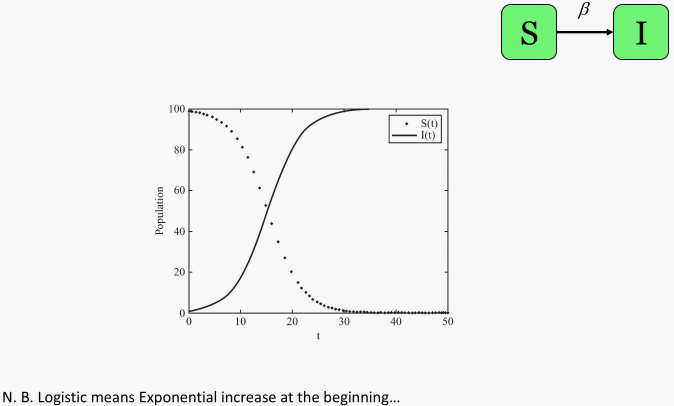
\includegraphics[width=0.5\linewidth]{figures/SI.png}
      \end{figure}
      Gli individui \textbf{suscettibili (S)} possono venire infetti, se \textbf{infetti (I)} non possono essere curati e possono infettare altri utenti. Sia $N$ la dimensione della \textbf{crowd}, costante:
      \begin{itemize}
          \item $S(t)$: numero di individui suscettibili all'istante $t$ - $s(t) = \frac{S(t)}{N}$;
          \item $I(t)$: numero di individui infetti all'istante $t$ - $\frac{I(t)}{N}$;
          \item $\beta$: probabilità di contatto - per $\beta=1$ tutti entrano in contatto con tutti, per $\beta=0$ nessuno entra in contatto con nessuno.
      \end{itemize}
      Dimensione della crowd è $N=S(t)+I(t)$, per ogni istante un individuo infetto può \textbf{incontrare} $\beta N$ individui e può \textbf{infettarne} $\beta S$, per gli altri $\beta I$ non succede niente, $\beta IS$ saranno infettati al prossimo istante.
      \begin{figure}[H]
          \centering
          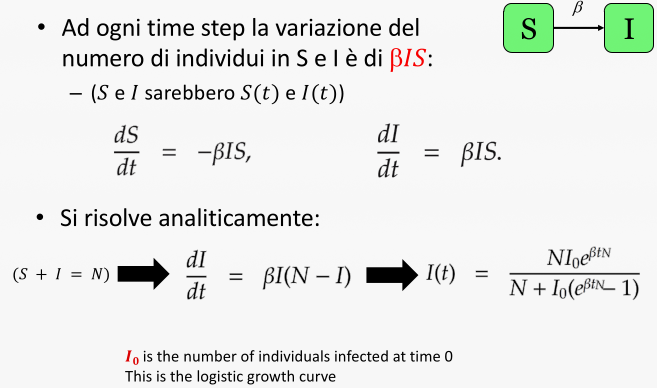
\includegraphics[width=0.6\linewidth]{figures/si_model.png}
      \end{figure}
  \subsection{SIR model}
    \begin{figure}[H]
        \centering
        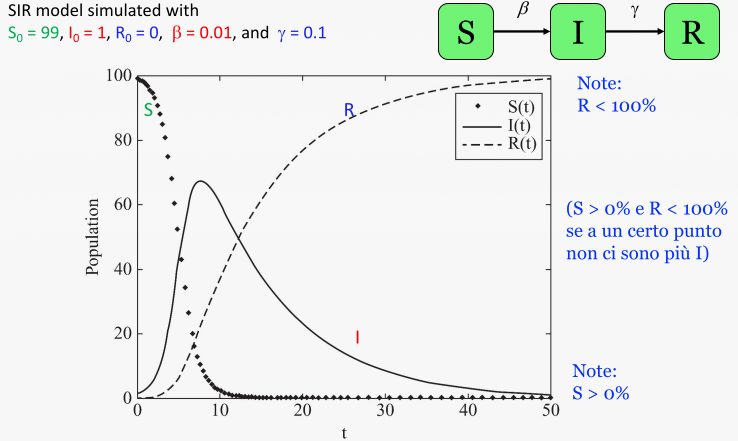
\includegraphics[width=0.5\linewidth]{figures/SIR.png}
    \end{figure}
    Introduce (in aggiunta a \textbf{I} e \textbf{S}) lo stato di \textbf{recovery R}: determinati individui possono "curarsi" (o essere rimossi / morire), una volta arrivato a stato \textbf{R} non può più tornare \textbf{I}.
    $$S+I+R=N$$
    $\gamma$ invece definisce la probabilità di recover di un individuo infetto ad un dato istante.
    \begin{itemize}
        \item S decrescono monotonicamente;
        \item R crescono monotonicamente;
        \item I crescono inizialmente e poi decrescono man mano che individui guariscono / muoiono e vanno a 0 per $t\rightarrow\infty$;
        \item S \textbf{non vanno} a 0: ne resta una generalmente piccola frazione (quando non ci sono più I non c'è nesusno per contagiare i pochi S che si salvano).
    \end{itemize}
    $R_0$ \textbf{Basic reproduction number} (calcolato con $\beta/\gamma$) numero medio di individui che un individuo infetta prima di guarire / morire. $R_0=1$ indica la \textbf{soglia epidemica}, quindi \textbf{c'è} epidemia se $R_0\geq1$, se $R_0\leq1$ non c'è epidemia perché gli infetti guariscono più in fretta di quanto gli S si ammalino.
    \subsubsection{Transizione epidemica}
      Transizione di fase fra regime epidemia e regime non-epidemia: brusca, improvvisa.
  \subsection{SIS model}
    \begin{figure}[H]
        \centering
        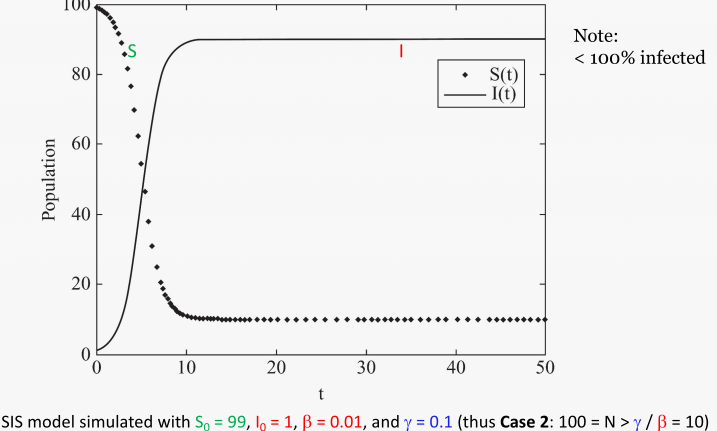
\includegraphics[width=0.5\linewidth]{figures/SIS.png}
    \end{figure}
    Uguale a modello SI, ma soggetti infetti possono tornare sani e venire ri-infettati di nuovo.
    $$I(\beta N-\gamma)-\beta I^2$$
    \begin{itemize}
        \item Se $\beta N\leq\gamma$: gli infetti diminuiranno esponenzialmente;
        \item Se $\beta N>\gamma$: crescita logistica simile al modello SI.
    \end{itemize}
  \subsection{SIRS model}
    \begin{figure}[H]
        \centering
        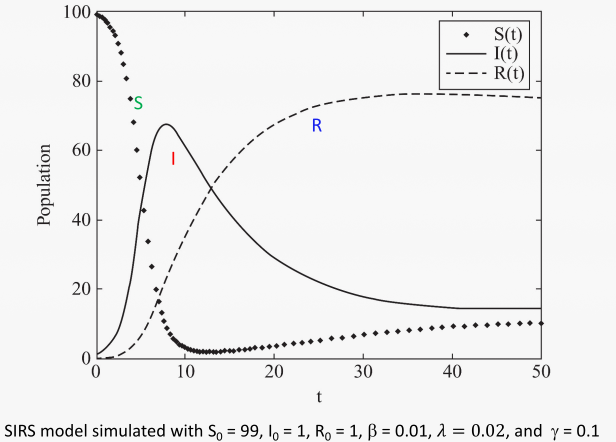
\includegraphics[width=0.3\linewidth]{figures/SIRS.png}
    \end{figure}
    Individui che sono in stato R perdono l'immunità dopo un certo periodo di tempo e diventano suscettibili di nuovo
  \subsection{Contagio sociale}
    Se un individuo vede un comportamento in un altro individuo, lo \textbf{imita} (adotta lo stesso comportamento), rappresentabile come \textbf{modifica di SIR}:
    \begin{itemize}
        \item Suscettibile - \textbf{Ignorant (I)}: individuo che non ha ancora ricevuto l'info;
        \item Infetto - \textbf{Spreader (S)}: individuo che ha ricevuto l'info e la diffonde;
        \item Recovered/Removed - \textbf{Stifler (R)}: ha ricevuto l'info ma non la diffonde (più).
    \end{itemize}
    A differenza di SIR (patologia \textbf{negativa}), il contagio sociale (ISR) è un atto intenzionale, vantaggioso ed attivo.
    \begin{figure}[H]
        \centering
        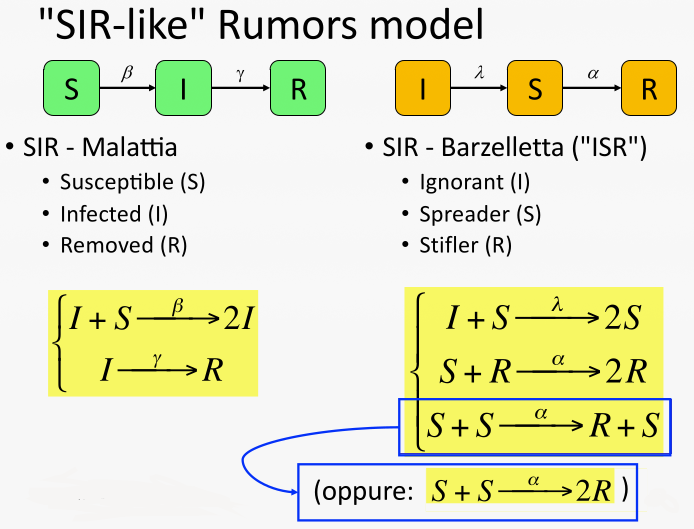
\includegraphics[width=0.4\linewidth]{figures/SIRISR.png}
    \end{figure}
    \begin{itemize}
        \item Passaggio $I \rightarrow R$ in SIR è spontaneo e dipende solo da n° di I e dal parametro $\gamma$;
        \item Passaggio $S \rightarrow R$ in "ISR" non è spontaneo e dipende da n° di S, parametro $\alpha$ e dal n° di R.
    \end{itemize}
    \subsubsection{Cosa succede}
      \begin{itemize}
        \item Allo \textbf{stato stazionario} ($t\rightarrow\infty$) non ci saranno più \textbf{spreaders} - $s_\infty=lim_{t\rightarrow\infty}s(t)=0$;
        \item Gli ignoranti saranno tanti di meno quanti di più saranno gli stiflers - $i_\infty=e^{-(1+\lambda/\alpha)r_\infty}$;
        \item Gli stiflers saranno tutti gli altri, $i_\infty+r_\infty=1$, $r_\infty=1-i_\infty$ - $r_\infty=1-e^{-(1+\lambda/\alpha)r_\infty}$.
      \end{itemize}
    \subsubsection{Condizione}
      Per avere contagio sociale la condizione diventa $1+\frac{\lambda}{\alpha}$. \textbf{Non c'è più soglia epidemica}, qualsiasi siano i valori dei parametri c'è \textbf{sempre} epidemia sociale.
\section{Epidemie su reti}
  Supponiamo di avere una \textbf{rete omogenea}, tutti i nodi hanno un grado simile e ogni individuo viene a contatto con lo stesso numero di individui. Si può ridefinire il \textbf{basic reproduction number} (n° di individui che un infected contagia prima di guarire / morire).
  \begin{itemize}
      \item \textbf{Rete omogenea}: tutti i nodi hanno grado simile alla media $<k>$;
      \item Ogni $I$ infetta un vicino $S$ con probabilità $\beta$;
      \item Ad inizio epidemia sono quasi tutti $S$, anche i vicini di un $I$;
      \item N° medio di infezioni causate da un $I$: $\beta<k>$;
      \item Ad ogni istante $t$, ogni $I$ può transitare in $R$ con probabilità $\gamma$.
  \end{itemize}
  Quindi:
  \begin{itemize}
    \item $\Delta I_{t+1} = \beta<k>I_t$;
    \item $\Delta R_{t+1} = \gamma I_t$.
  \end{itemize}
  Per avere epidemia deve essere $\Delta I_{t+1} > \Delta R_{t+1}$, ossia $\beta<k>I_t > \gamma I_t$. \textbf{Quindi} $R_0 = <k>\beta/\gamma$.
  \subsection{Intervention}
    Per diminuire $R_0$:
    \begin{itemize}
        \item Diminuire \textbf{contagiosità} $\beta$;
        \item Aumentare \textbf{velocità di guarigione} $\gamma$;
        \item Diminuire il \textbf{grado medio} $<k>$.
    \end{itemize}
  Nel \textbf{mondo reale} reti sono eterogenee (power law, hub), se ci sono nodi con grado alto non c'è soglia e c'è comunue un'epidemia (hub si contagiano facilmente e contagiano molti altri).
  \subsection{Epidemic intervention}
    Scelgo nodi randomici e gli chiedo di selezionare gli altri individui più suscettibili, studio sperimentale su \textbf{rete WSSW}:
    \begin{itemize}
        \item $\lambda=\alpha=1$;
        \item non fully mixed (\textbf{non completa});
        \item variazione rispetto a probabilità $p$:
          \begin{itemize}
              \item per $p$ \textbf{bassi} - rete molto clusterizzata, alto $C$ e molti triangoli, spreaders diffondono sempre agli stessi e quindi passano velocemente fra stiflers (poca diffusione);
              \item per $p$ \textbf{alti} - rete con shortcut, spreaders diffondono anche in parti lontane e quindi rumor si diffonde.
          \end{itemize}
    \end{itemize}
  \subsection{Su reti eterogenee}
    Power law, scale-free, con hub e \textbf{varianza alta} sui gradi. Hub dovrebbero essere spreader efficientissimi, tuttavia $r_\infty$ è più alto su reti omogenee... infatti hub non aiutano diffusione per i rumor: facile che un rumor raggiunga un hub (rendendo diffusione molto alta), ma se hub diventa spreader allora creerà velocemente molti \textbf{molti stifler}.
\section{Modello dei benefici diretti (Morris)}
  Persone sono influenzate da altre persone sulla base di \textbf{informazioni} (faccio X perché vedo molti che lo fanno) e \textbf{benefici diretti} (faccio X perché mi conviene rispetto a non farlo).
  \subsection{Modello direct benefit}
    Comportamento si diffode sulla rete sulla base di un processo di decision making basato su scelte dei nodi vicini.
  \subsection{Modello di Morris}
    Valuto un nodo di partenza e valuto i nodi vicini, per un nodo il \textbf{beneficio} di adottare un comportamento cresce al crescere del n° dei vicini che lo adottano. Ogni nodo sceglie fra due possibili comportamenti \textit{A} e \textit{B}, se due nodi $v$ e $w$ sono collegati da un arco hanno un incentivo ad \textbf{adottare comportamenti uguali}.
    \subsubsection{Matrice payoff}
      \noindent
        \begin{minipage}[c]{0.58\linewidth}
            $v$ e $w$ \textbf{giocatori}, $A$ e $B$ \textbf{strategie}:
            \begin{itemize}
                \item se $v$ e $w$ adottano entrambi $A$ allora \textbf{payoff} $a>0$;
                \item se $v$ e $w$ adottano entrambi $B$ allora \textbf{payoff} $b>0$;
                \item se $v$ e $w$ adottano comportamenti differenti allora \textbf{payoff} 0;
            \end{itemize}
        \end{minipage}
        \hfill
        \begin{minipage}[c]{0.38\linewidth}
            \centering
            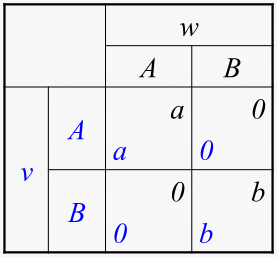
\includegraphics[width=0.8\linewidth]{figures/payoff.png}
        \end{minipage}
      Ogni nodo seleziona strategia che massimizza la somma di tutti i payoff (trovati creando la matrice con tutti i suoi vicini).
    \subsubsection{Regola di decisione}
      Decisione della strategia dipende da:
      \begin{itemize}
          \item payoff $a$;
          \item payoff $b$;
          \item n° vicini che adottano $A$ (basta anche percentuale);
          \item n° vicini che adottano $B$ (basta anche percentuale);
          \item $p$ = percentuale vicini che adottano A, 1-p = percentuale vicini che adottano B;
          \item $d$ = n° vicini.
      \end{itemize}
      Se $v$ adotta $A$ payoff = $pda$, se adotta $B$ payoff = $(1-p)db$. $v$ adotta $A$ \textbf{se e solo se} $pda\geq(1-p)db$, ossia se $p\geq\frac{b}{a+b}$.
    \subsubsection{Equilibri}
      2 ovvi equilibri (tutti A / tutti B), definendo inizialmente un \textbf{comportamento di default}, ci sono poi \textbf{early adopters} che vanno contro il comportamento default per ragioni extra-payoff. Ad ogni passo ogni nodo usa la \textbf{regola di decisione} per per scegliere se cambiare comportamento, si ferma quando tutti sono cambiati / nessuno vuole più cambiare. Si ha quindi una \textbf{cascata di adozioni} e, se tutti i nodi passano a un singolo comportamento si ha \textbf{cascata completa}.
    \subsubsection{Intervention}
      Strategie che possono essere usate per cambiare le decisioni, \textbf{miglioando i payoff} o \textbf{convincendo} alcuni nodi chiave per far ripartire la reazione a catena.
    \subsubsection{Risultato di Morris}
      Se esistono \textbf{cluster} (comunità molto legate con sottografi quasi completi e poco legati all'esterno) \textbf{ferman le cascate}, in particolare una cascata si ferma \textbf{se e solo se} c'è un cluster.
      \begin{itemize}
          \item Dati degli \textbf{initial adopters} di $A$;
          \item Si definisce \textbf{soglia} $q$ per adottare $A$;
          \item Se il resto della rete contiene un cluster di \textbf{densità} $> 1-q$ allora non ci sarà una cascata completa;
          \item Se non c'è cascata completa, allora c'è un \textbf{cluster} di densità $> 1-q$.
      \end{itemize}
      \textbf{Dimostrazioni}
      \begin{itemize}
          \item Caso 1:
            \begin{itemize}
                \item Sia un cluster con densità $> 1-q$, sia $v$ il \textbf{primo} nodo nel cluster che adotta $A$ (al tempo $t$);
                \item A $t-1$ doveva esserci almeno una frazione $q$ di vicini di $v$ adottanti $A$, nessuno \textbf{nel} cluster adottava $A$;
                \item $v$ aveva almeno una frazione $q$ di vicini fuori dal cluster;
                \item Il cluster è di densità $> 1-q \rightarrow > 1-q$ vicini di $v$ devono essere nel cluster;
                \item Impossibile averne $q$ fuori... \textbf{no complete cascade}.
            \end{itemize}
          \item Caso 2:
            \begin{itemize}
                \item Sia un qualsiasi nodo $w$ in $S$;
                \item $w$ non cambia da $B$ ad $A$, la frazione dei suoi vicini che usano $A$ è $F_W(A) < q$ e la frazione dei suoi vicini che usano $B$ è $F_W(B) > 1-q$;
                \item Soli nodi che usano $B$ sono quelli in $S$, la frazione dei vicini di $w$ che stanno in $S$ è $> 1-q$;
                \item Questo vale per tutti i nodi $w$ in $S$, per ognuno di questi la frazione dei vicini che stanno in $S$ è $> 1-q$ e quindi $S$ è un \textbf{cluster} di densità $> 1-q$.
            \end{itemize}
      \end{itemize}
      \begin{figure}[H]
          \centering
          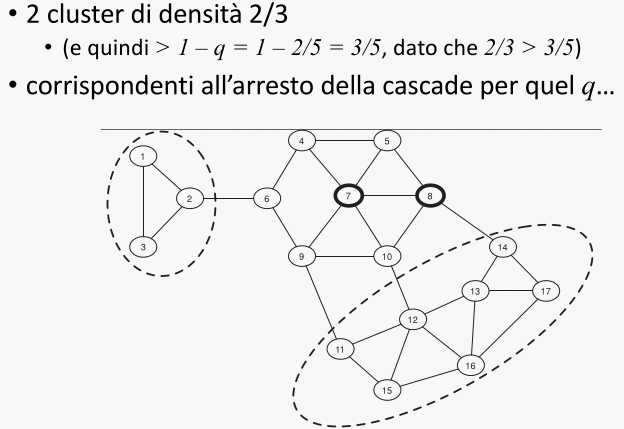
\includegraphics[width=0.4\linewidth]{figures/morris_es.png}
      \end{figure}
    \subsubsection{Awareness, adoption, weak ties}
      \textbf{Weak ties} sono utili per conoscenze non intime (es. trovare lavoro), utili pere diffusione informazioni ma inutili per diffusione mode, innovazione. Ricorsiao che \textbf{awareness} = semplice consapevolezza e \textbf{adoption} = adozione comportamento. Posso estendere il modello di Morris con \textbf{payoff eterogenei}:
      \begin{itemize}
          \item Ogni nodo $v$ ha una ricompensa diversa $a_v$ ($b_v$) per l'adozione del comportamento $A$ ($B$)
          \item Modellando così non solo chi è \textbf{influente} ma anche chi è \textbf{facilmente influenzabile}.
      \end{itemize}
      \begin{figure}[H]
          \centering
          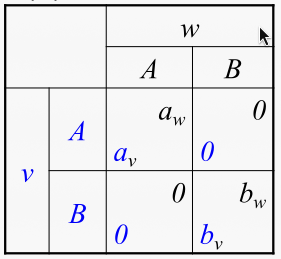
\includegraphics[width=0.3\linewidth]{figures/morris_est.png}
      \end{figure}
\section{Fake news}
  Quando parliamo di \textbf{fake news} parliamo di:
  \begin{itemize}
      \item \textbf{misinformation} = errori non intenzionali come diffusione di informazioni sbagliate "\textbf{in buona fede}";
      \item \textbf{disinformation} = diffusione di contenuti / informazioni volutamente manipolate;
      \item \textbf{malinformation} = diffusioni di info malevole con intenti diffamatori.
  \end{itemize}
  Un'informazione si valuta sotto \textbf{7 dimensioni}:
  \begin{itemize}
      \item \textbf{correctness} - informazione espressa in maniera accurata senza sbagli;
      \item \textbf{neutrality} - informazione espressa sotto punto di vista oggettivo / neutrale;
      \item \textbf{comprehensibility} - informazione comprensibile / capibile / leggibile facilmente);
      \item \textbf{precision} - informazione è precisa / specifica, non vaga;
      \item \textbf{completeness} - informazione è completa e racconta "tutta la storia";
      \item \textbf{speaker's trustworthiness} - chi trasmette informazione è generalmente affidabile;
      \item \textbf{indormativeness} - informazione permette di ricavare dati utili.
  \end{itemize}
  \subsection{Perché studiarle}
    Fenomeno in forte crescita e sempre più problematico senza soluzione ovvia, studi hanno evidenziato che notizie false si diffondono quasi allo stesso rateo delle vere, ma con depth e size maggiore.
    \begin{itemize}
        \item Si è notato come notizie false vengano pubblicate con \textbf{più frequenza} delle vere, e come causino paura, disgusto e sorpreasa per restare impresse;
        \item Anche se implementassimo un \textbf{bot} per diffonderle non cambierebbe niente in quando vengono diffuse maggiormente da \textbf{umani};
        \item Due comunità ben distinte (buona parte dei post ha \textbf{alta omogeneità}): \textbf{cospirazionisti} e \textbf{scientifici}, che scaturiscono nelle \textbf{echo chambers} ad alta omogeneità (contenuti tendono a circolare solo all'interno della rispettiva comunità);
        \item Si è riscontrato come attività di \textbf{debunking} sembra inutile (se non controproducente) a causa di \textbf{pregiudizio di conferma (confirmation bias)}: si crede a quello che si sa già.
    \end{itemize}
\section{Crowdsourcing}
  Sistemi computazionali vengono supportati dal \textbf{comportamento sociale}: compiti che i calcolatori non fanno bene svolti da persone raggounte tramite i sistemi computazionali. Si sfruttano quindi le \textbf{folle} (possono avere comportamenti positivi / negativi), solitamente decisioni prese da un gruppo sono \textbf{più corrette} di quelle dei singoli esperti. Si parla quindi di \textbf{decisioni di gruppo}.
  \subsection{4 elementi perché "funzioni"}
    \begin{itemize}
        \item \textbf{Diversità di opinioni}: ognuno deve avere le proprie \textbf{informazioni private} (al limite un'interpretazione originale dei fatti noti);
        \item \textbf{Indipendenza}: le opinioni personali \textbf{non sono determinate} dalle opinioni di chi sta intorno (\textit{no herding behavior, cascade});
        \item \textbf{Decentralizzazione}: persone sono capaci di \textbf{specializzare e basarsi su conoscenze locali};
        \item \textbf{Aggregazione}: esistono meccanismi per \textbf{trasformare giudizi privati in una decisione collettiva}.
    \end{itemize}
  \subsection{5 motivi per cui non sempre "funziona"}
    \begin{itemize}
        \item \textbf{Omogeneità}: necessità che ci sia \textbf{diversità} in una folla, per avere abbastanza varietà di approcci / ragionamenti / informazioni private;
        \item \textbf{Centralizzazione}: disastro dello shuttle Columbia attribuibile alla \textbf{gestione gerarchica / burocratica} della nasa (chiusa rispetto a ingegneri di "basso livello");
        \item \textbf{Divisione}: informazioni \textbf{appartenenti a una sottodivisione non accessibili alle altre} (torri gemelle). Folle lavorano meglio se scelgono autonomamente su cosa lavorare e con quali informazioni;
        \item \textbf{Imitazione}: scelte \textbf{visibili ed effettuate in sequenza}, si può formare una \textbf{information cascade} (\textit{herding behavior}) in cui solo prime scelte vengono fatte in modo genuino e poi si tende a confermare / copiare;
        \item \textbf{Emotività}: fattori \textbf{emotivi} possono portare a pressioni, \textit{istinto di gregge} e, in casi estemi, a \textbf{isteria collettiva}.
    \end{itemize}
  \subsection{Definizione}
    Compito tipicamente svolto da uno / pochi dipendenti esperti viene svolto in \textbf{outsourcing} con un \textbf{grande} gruppo di persone / community mediante una \textbf{chiamata aperta}.
  \subsection{Human computation}
    Processo computazionale che da in outsourcing \textbf{alcuni passi} ad umani: computer chiede a persona / crowd di risolvere un problema, lo raccoglie, interpreta e integra le soluzioni (reCAPTCHA).
  \subsection{Esempi reali}
    \begin{itemize}
        \item Ricercatore che vuole dati epr esperimenti;
        \item Azienda che vende beni (indagini di mercato veloci e a basso prezzo);
        \item Amministrazione comunale che vuole sapere presenza di buche nelle strade.
    \end{itemize}
  \subsection{Amazon mechanical turk}
    Mercato che richiede intelligenza umana per del lavoro dove i player sono:
    \begin{itemize}
        \item \textbf{requester} - individuo / organizzazione con lavoro da far svolgere;
        \item \textbf{worker} - persona che fa il lavoro;
        \item \textbf{HIT} (Human Intelligence Task) - unità di lavoro da svolgere alla quale è associato un pagamento;
        \item \textbf{batch} - insieme di HIT caricato da un requester.
    \end{itemize}
    L'esito di un HIT o di un batch può venire rappresentato mediatnte una \textbf{matrice $n$ task / $m$ worker}, con $v_{ij}$ valori dati in risposta dal worker $i$ per la task $j$ (numero / testo / ...).
    \begin{figure}[H]
        \centering
        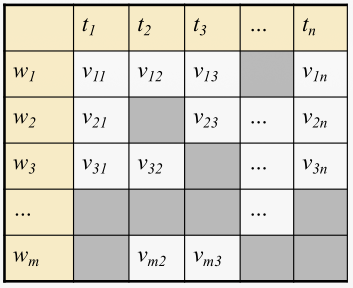
\includegraphics[width=0.3\linewidth]{figures/m_wo_ta.png}
    \end{figure}
    La matrice è \textbf{sparsa}: non tutti i worker fanno tutti i task e non tutti i task sono fatti da tutti i worker.
    \subsubsection{Principi di Surowiecki}
      Amazon mechanical turk rispetta i 4 principi di Surowiecki: diversità di opinioni, indipendenza, decentralizzazione e aggregazione.
  \subsection{Tipi di task}
    \begin{itemize}
        \item \textbf{Complex task}: creazione website, sviluppo sistema SW;
        \item \textbf{Simple projects}: sviluppare logo / visual identity;
        \item \textbf{Macro tasks}: scrivere recensione, testare una feature nuova;
        \item \textbf{Micro tasks}: labelling di un'immagine, verificare un indirizzo.
    \end{itemize}
    \subsubsection{Demartini}
      Classificazione (capitoli) basata sulla \textbf{letteratura scientifica} in vari settori di ricerca, \textbf{sistemi ibridi} (human + machine) per:
      \begin{itemize}
          \item DB;
          \item information retrieval;
          \item processing di linguaggio naturale;
          \item semantic web;
          \item machine learning;
          \item multimedia processing.
      \end{itemize}
    \subsubsection{Brabham}
      4 tipi di task sulla base dei problemi risolti:
      \begin{itemize}
          \item \textbf{Knowledge discovery and management} - scoprire e organizzare / gestire conoscenze\textbf{già disponibili} ma \textbf{disorganizzate}, utile per raccolta e organizzazione info, creazione risorse collettive e reporting;
          \item \textbf{Broadcast search} - trovare uno \textbf{specialista} (spesso fuori dal settore - "mente fresca") che svolga il compito, trovi la risposta giusta e dia la soluzione, utile per problemi tecnico-scientifici con soluzioni misurabili;
          \item \textbf{Peer-vetted creative production} - produzione creativa riesaminata da pari, \textbf{crowd} produce e seleziona idee creative (sensato perché sarà massa ad usarle), utile per problemi la cui soluzione dipende da gusti e/o mercato;
          \item \textbf{Distributed human-intelligence task} - grandi problemi di data processing decomposti in piccoli task che richiedono intelligenza umana (Amazon mechanical turk), utile per analisi dati su larga scala.
      \end{itemize}
    \subsubsection{Grier}
      Classificazione più articolata con tipi di pagamento e tipi di mercato:
      \begin{itemize}
        \item Crowd\textbf{contest}: do in \textbf{outsourcing} un compito intero (solitamente) senza scomporlo, mediante un \textbf{contest} dove si seleziona e si paga \textbf{solo} la risposta migliore (es. design di un logo);
        \item \textbf{Macro}tasking: dare in \textbf{outsourcing} a un consulente / libero professionista, pagamento orario (es. traduzioni, creazione app);
        \item \textbf{Micro}tasking: compito \textbf{suddiviso} in piccole parti, poi aggregate (\textbf{il vero Crowdsourcing});
        \item \textbf{Self-organized crowds}: chiedo che venga svolto un lavoro ma gli individui \textbf{cooperano / interagiscono}.
        \item Crowd\textbf{funding}: non si vuole lavoro ma soldi, tante piccole donazioni (gofundme).
      \end{itemize}
      2 tipi di pagamento:
      \begin{itemize}
          \item \textbf{Pay-all}: tutti i worker che hanno svolto il lavoro vengono pagati (tipico);
          \item \textbf{Pay-one}: solo uno viene pagato (contest).
      \end{itemize}
      2 tipi di mercato / crowd:
      \begin{itemize}
          \item \textbf{Indipendenti}: ognuno lavora per sé e viene pagato individualmente;
          \item \textbf{Collaborative}: cooperazione fra i worker, a volte si dividono la paga.
      \end{itemize}
      \begin{figure}[H]
          \centering
          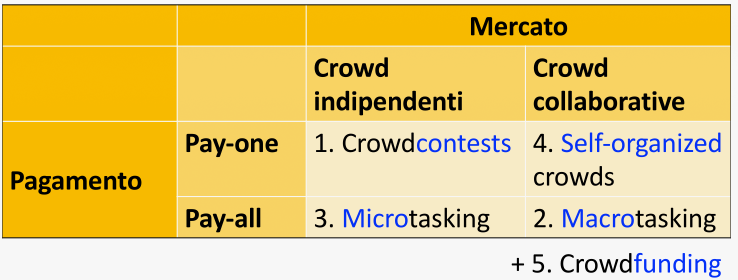
\includegraphics[width=0.6\linewidth]{figures/grier.png}
      \end{figure}
  \subsection{Come convincere i worker}
    2 tipi di motivazioni:
    \begin{itemize}
        \item \textbf{Estrinseche}: compito considerato noioso, inutile o spiacevole necessita di \textbf{ricompensa aggiuntiva} (soldi, fama, reputazione, il mio tesoro, cercatelo, chissà se qualcuno di voi lo troverà);
        \item \textbf{Intrinseche}: attività consegue a interesse / divertimento del compito stesso, la ricompensa è quindi \textbf{intrinseca} nello svolgimento del compito (Games With A Purpose).
    \end{itemize}
    \subsubsection{Li et al}
      Classificazione \textbf{bidimensionale} che mette isieme \textbf{granularità} (microtask / macrotask) e \textbf{incentivo / motivazione} (denaro / divertimento).
      \begin{figure}[H]
          \centering
          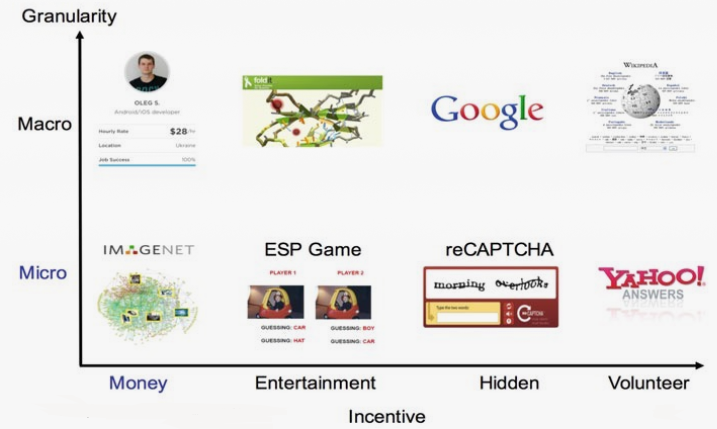
\includegraphics[width=0.4\linewidth]{figures/li_et_al.png}
      \end{figure}
  \subsection{Tipi di risposte}
    Domande a risposta singola / multipla, risposta aperta numerica / testuale, collection di dati. 
    \subsubsection{Real world tasks}
      Sempre con associazione \textbf{task - tipo di risposta} con:
      \begin{itemize}
          \item \textbf{sentiment analysis} - opinione di una review;
          \item \textbf{search relevance} - data un'interrogazione dire se un documento è pertinente con 2 o N valori;
          \item \textbf{moderazione contenuti} - immagini o siti web, risposta singola S/N;
          \item \textbf{raccolta dati} - points of interest / coordinate geografiche;
          \item \textbf{categorizzazione} - ad es. classificare come attore o come cantante;
          \item \textbf{trascrizione di audio / immagini} - digitalizzazione con dati immediatamente usabili.
      \end{itemize}
      Esito di un esperimento di crowdsourcing rappresentabile sempre mediante una \textbf{matrice worker / task}.
      \begin{figure}[H]
          \centering
          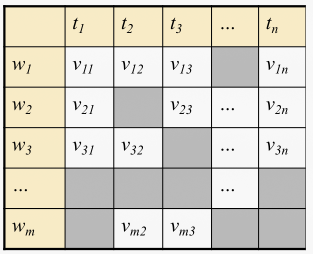
\includegraphics[width=0.3\linewidth]{figures/m_r_w_t.png}
      \end{figure}
\section{Progettare microtask}
  \begin{figure}[H]
      \centering
      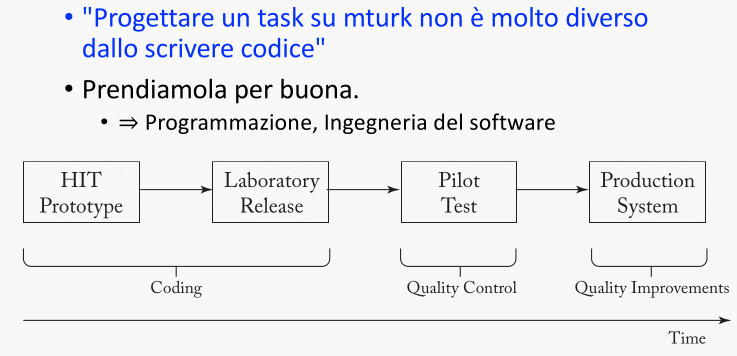
\includegraphics[width=0.6\linewidth]{figures/task_def.png}
  \end{figure}
  Il workflow per la definizione di una task si suddivide in 6 parti:
  \begin{enumerate}
      \item \textbf{Definire il problema}: comprenderlo per bene in modo da non risolvere il problema sbagliato;
      \item \textbf{Idea di soluzione}: capire che esperimento effettuare con un progetto vero e proprio (cosa mostrare / chiedere su quanti / quali dati, con quanta ridondanza, quanto pagare e quali controlli di qualità effettuare), fornendo \textbf{istruzioni chiare} e raccogliendo \textbf{feedback};
      \item \textbf{Prototipo di HIT}: imolementazione di tutto, magari non su tutti i dati e non con tutti i controlli (anche versioni alternative);
      \item \textbf{Rilascio in laboratorio}: far svolgere il compito ad alcuni collaboratori per capire se ci sono \textbf{bug} e iniziare a imbastire la fase di analisi dati;
      \item \textbf{Test pilota}: far svolgere il compito sulla piattaforma con worker e soldi \textbf{veri} su un insieme \textbf{fittizio / limitato} di dati oer comprendere scalabilità e collaudare GUI, istruzioni...;
      \item \textbf{In produzione}: lancio esperimento finale con precauzioni, è difficile avere risposte perfette ed esatte.
  \end{enumerate}
  La qualità perfetta dei dati ottenuti mediante crowdsourcing è un'\textbf{utopia}, ci sono errori, incongruenze ecc. \textbf{Si fa il meglio che si può con i dati che si ha}.
\section{Qualità}
  \subsection{Tecniche per migliorare / ottenere buona qualità}
    \subsubsection{Task design}
      Scelte progettuali (pairwise vs singolo), modalià di presentazione, worker nelle migliori condizioni possibili ma \textbf{controlli costanti}.
    \subsubsection{Qualification test}
      Valutazioni prima del task: se un worker vuole svolgere un task deve prima superare un \textbf{test esplicito} (worker sa che sta facendo un test). Voglio selezionare worker \textbf{qualificati} e motivati a superare il test (magari senza paga). Il test può esseresa \textbf{piattaforma} o \textbf{interno} al task (prime domande).
    \subsubsection{Controlli sintattici}
      Parsing dell'input / preprocessing per evitare \textbf{campi vuoti} (matrici sparse), ma anche conteggio caratteri / parole e parsing più sofisticati e \textbf{controlli anti copiatura}.
    \subsubsection{Testi nascosti}
      \textbf{Nascosti} nelle varie parti del task, domande per definire qualità del worker (spesso facili o di cui si sa già la risposta) e spesso \textbf{ripetute} per valutare coerenza.
    \subsubsection{Monitoraggio tempi}
      Verifica del tempo impiegato per leggere istruzioni e compito, sia su singole parti che su totale: se troppo o troppo poco il worker viene scartato.
    \subsubsection{Monitoraggio azioni}
      Valutazione spostamenti mouse, focus, scrolling, click, ordine inserimento dati, pattern di navigazione fra pagine, mediante \textbf{behavioral logger}.
    \subsubsection{Controlli ex post}
      Il worker ha finito il task e sottomesso il risultato, posso decidere di:
      \begin{itemize}
          \item non usarli (pagandolo);
          \item non accettarli (non pagarlo - quando non pago cala mia reputazione come requester);
          \item non pagarlo e bloccarlo (impedendogli di fare altri task dello stesso batch).
      \end{itemize}
  \subsection{Ridondanza e aggregazione}
    Raccogliere più vlte lo stesso dato dalla stessa domanda e poi aggregare in un unico dato è una tecnica al cuore del crowdsourcing. La misura della qualità si divide quindi in:
    \begin{itemize}
        \item \textbf{qualità individuale} della risposta di un singolo worker;
        \item \textbf{qualità aggregata} delle risposte a un task;
        \item \textbf{qualità di un worker}: qualità media delle sue risposte.
    \end{itemize}
    \subsubsection{Qualità individuale}
      \noindent
        \begin{minipage}[c]{0.48\linewidth}
            Si ripende la matrice \textbf{workers / tasks} aggiungendoci la \textbf{verità}: singola e nota come unico valore corretto.
        \end{minipage}
        \hfill
        \begin{minipage}[c]{0.48\linewidth}
            \centering
            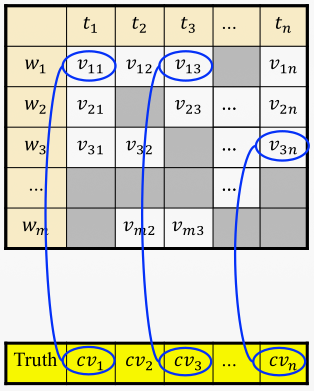
\includegraphics[width=0.7\linewidth]{figures/qua_ind.png}
        \end{minipage}
    \subsubsection{Qualità aggregata}
      \noindent
        \begin{minipage}[c]{0.48\linewidth}
            Dopo aver aggregato tutte le risposte a un task in un valore unico (mediante media, mediana, moda...). \textbf{Qualità aggregata > qualità individuale}, è proprio l'idea del crowdsourcing.
        \end{minipage}
        \hfill
        \begin{minipage}[c]{0.48\linewidth}
            \centering
            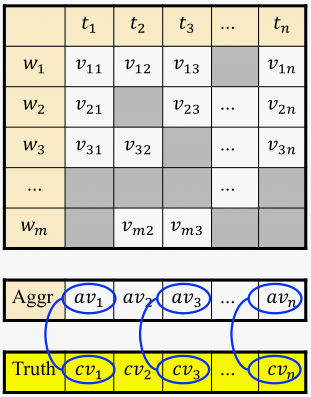
\includegraphics[width=0.7\linewidth]{figures/qua_agg.png}
        \end{minipage}
    \subsubsection{Più formalmente}
      \begin{figure}[H]
          \centering
          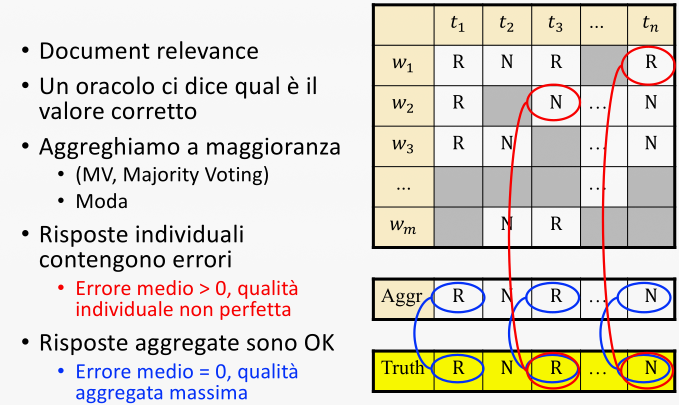
\includegraphics[width=0.3\linewidth]{figures/qua_for.png}
      \end{figure}
      \begin{itemize}
          \item $w_i \in W = \{w_i\}_{i=1 \dots m}$: $i$-esimo worker, e l'insieme dei worker;
          \item $t_j \in T = \{t_j\}_{j=1 \dots n}$: $j$-esimo task, e l'insieme dei task;
          \item $v_{ij}$: i valori (le risposte) dati dal worker $i$ al task $j$. Risposta mancante: $\bot$;
          \item $W_j = \{w_i \in W \mid v_{ij} \neq \bot\}$: l'insieme dei worker che hanno risposto al task $t_j$;
          \item $T_i = \{t_j \in T \mid v_{ij} \neq \bot\}$: l'insieme dei task a cui ha risposto il worker $w_i$;
          \item $av_j = \text{F}_{agg}(\{v_{ij} \mid w_i \in W_j\})$: i valori aggregati per il task $t_j$;
          \item $cv_j$: i valori corretti (\textit{correct values}) per il task $t_j$.
      \end{itemize}
      \textbf{Similitudine media} con ground truth dei valori indivisuali è \textbf{minore} di quella dei valori aggregati:
      $$\frac{1}{n}\sum_{i=1}^n(\frac{1}{m}\sum_{i=1}^msim(v_{ij},cv_j)) < \frac{1}{n}\sum_{j=1}^nsim(av_j,cv_j)$$
      $$\frac{1}{n}\sum_{j=1}^n(\frac{1}{\abs{W_j}}\sum_{i\mid w_i\in W_j}sim(v_{ij},cv_j)) < \frac{1}{n}\sum_{j=1}^nsim(av_j,cv_j)$$
    \subsubsection{Funzioni di aggregazione}
      $$av_j = F_{aggr}({v_{ij} \mid w_j \in W_j}) = F_{aggr}({v_{ij} \mid v_{ij} \neq \bot})$$
      Possibili funzioni di aggregazione:
      \begin{itemize}
          \item Moda a maggioranza;
          \item Media aritmetica;
          \item Media geometrica;
          \item Media armonica;
          \item Mediana.
      \end{itemize}
    \subsubsection{Esempio aggregazione}
      \begin{figure}[H]
          \centering
          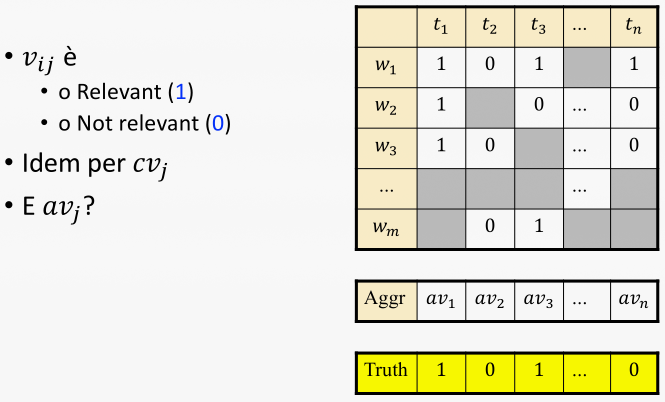
\includegraphics[width=0.6\linewidth]{figures/agg_es_1.png}
      \end{figure}
      \noindent
        \begin{minipage}[c]{0.68\linewidth}
            \begin{itemize}
                \item Moda (MV);
                \item + valori ammissibili;
                \item - perso informazioni.
            \end{itemize}
        \end{minipage}
        \hfill
        \begin{minipage}[c]{0.28\linewidth}
            \centering
            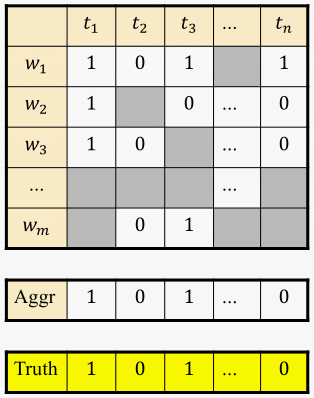
\includegraphics[width=\linewidth]{figures/agg_es_2.png}
        \end{minipage}
      \noindent
        \begin{minipage}[c]{0.68\linewidth}
            \begin{itemize}
                \item Media aritmetica;
                \item - valori non ammissibili;
                \item + perdo meno informazioni.
            \end{itemize}
        \end{minipage}
        \hfill
        \begin{minipage}[c]{0.28\linewidth}
            \centering
            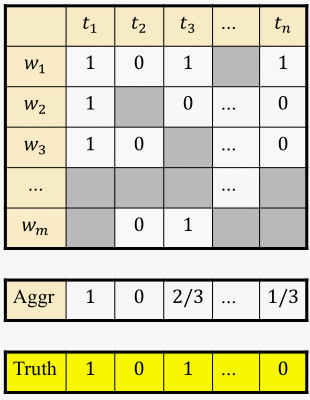
\includegraphics[width=\linewidth]{figures/agg_es_3.png}
        \end{minipage}
\section{Misurazione}
  Determinare una relazione fra una quantità ed un'unità di misura (\textbf{assegnare numeri a oggetti / eventi}), studiato nella \textbf{Measurement theory}.
  \subsection{Definizione 1}
    Assegnamento $w \in \Omega$ ($\Omega$ denota il set di tutti i possibili assegnamenti) è una funzione che assegna valori a oggetti in un set di oggetti $D$:
    $w : D \rightarrow \mathbb{R}$
    Posso avere diverse misure per la stessa cosa (metri vs pollici), posso cassificare \textbf{in colori} (non funziona benissimo), posso fare \textbf{aggregazioni} (temp media ultimi x gg).
  \subsection{Definizione 2}
    Assegnamento deve essere \textbf{omomorfo}: sia $<D,R_D>$ una struttura relazionale empirica e $<\mathbb{R},R_\mathbb{R}>$ una struttura relazionale numerale, una misurazione $\psi \in \Psi$ è un assegnamento di oggetti in un set $D$ (si denota con $\Psi \subset \Omega$ il set di tutti i misuramenti possibili):
    $$\psi : D \rightarrow \mathbb{R}$$
    $\forall x,y \in D (R_D(x,y) \implies R_\mathbb{R}(\psi(x),\psi(y)))$
    \noindent
      \begin{minipage}[c]{0.48\linewidth}
          \centering
          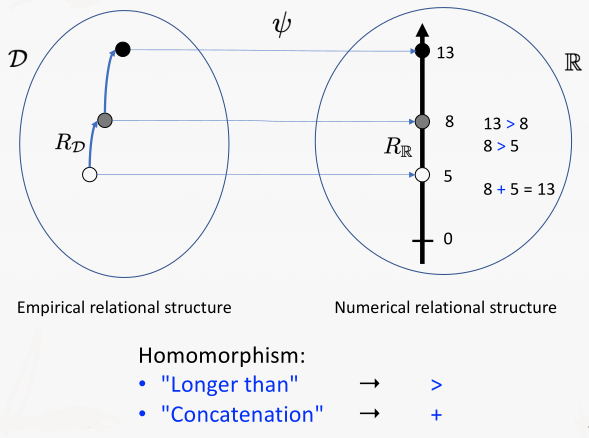
\includegraphics[width=0.8\linewidth]{figures/meas_es1.png}
      \end{minipage}
      \hfill
      \begin{minipage}[c]{0.48\linewidth}
          \centering
          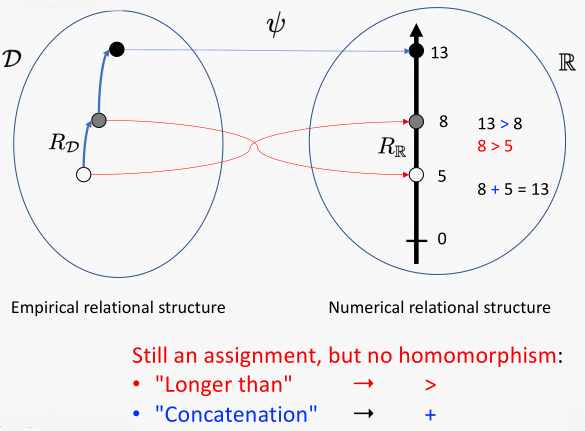
\includegraphics[width=0.8\linewidth]{figures/meas_es2.png}
      \end{minipage}
  \subsection{Scale di misura}
    \subsubsection{Ratio scale}
      Scala a \textbf{rapporti} "sono il doppio più alto di lui", poco efficiente per le date.
      $$y = f(x),  f(x) = a * x,  a > 0$$
    \subsubsection{Interval scale}
      Scala a \textbf{intervalli} "negli ultimi 2 giorni c'è stato un aumento di 5°C della temperatura", funziona per le date.
      $$y = f(x),  f(x) = ax + b,  a > 0$$
    \subsubsection{Ordinal scale}
      Una misutazione non è un valore ma un \textbf{rango} (funziona a classifica), $y = f(x)$ con f monotona crescente.
    \subsubsection{Nominal scale}
      Quantitativa e relativa a categorie, può essere \textbf{dicotomica} o no, non ci sono valutazioni su ratei, distanze, ranghi, $y = f(x)$  con f iniettiva.
    \subsubsection{Recap}
      \begin{figure}[H]
          \centering
          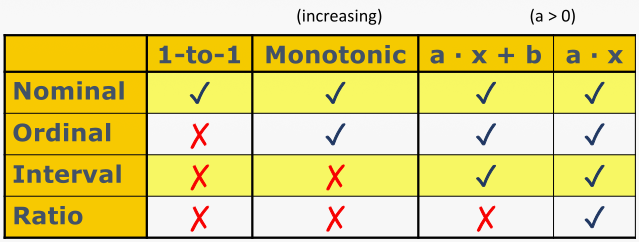
\includegraphics[width=0.6\linewidth]{figures/trasf_recap.png}
      \end{figure}
    \subsubsection{Operazioni ammissibili}
      \textbf{Data una scala}, solo alcune operazioni hanno senso (sono \textbf{legittime}):
      \begin{itemize}
          \item Relazionali: =, $\neq$, >, <;
          \item Aritmetiche: +, -, $\times$, /;
          \item Statistiche: media, mediana, moda.
      \end{itemize}
      \noindent
        \begin{minipage}[c]{0.48\linewidth}
            \centering
            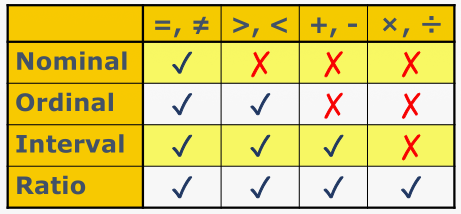
\includegraphics[width=\linewidth]{figures/leg_op.png}
        \end{minipage}
        \hfill
        \begin{minipage}[c]{0.48\linewidth}
            \centering
            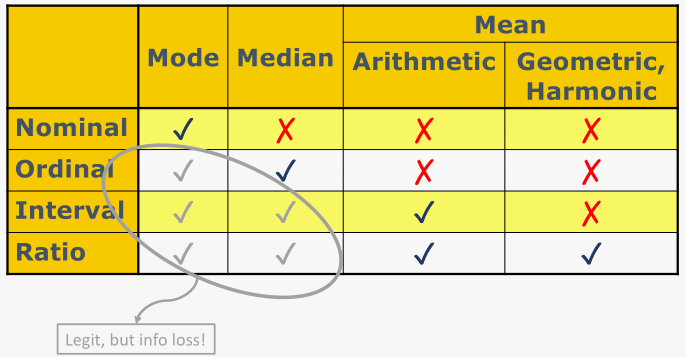
\includegraphics[width=\linewidth]{figures/leg_stat.png}
        \end{minipage}
  \subsection{Aggregazione Reloaded}
    Quando si aggregano giudizi su scale complesse (non binarie), sorgono problemi legati alla perdita di informazione e alla scelta della funzione corretta.
    \subsubsection{Il problema delle Scale Ordinali}
      Se abbiamo giudizi su scala ordinale (es. scala Likert a 6 valori: \textit{Pants on Fire} ... \textit{True}), l'approccio standard prevede l'uso della \textbf{Moda} o del \textbf{Majority Vote}. Tuttavia:
      \begin{itemize}
          \item \textbf{Perdita di informazione}: Una situazione con 51\% \textit{True} e 49\% \textit{Mostly True} viene trattata come 51\% \textit{True} e 49\% \textit{False}. La moda ignora la distribuzione dei voti "perdenti".
          \item \textbf{Magnitudine dell'errore}: Errori piccoli dovrebbero pesare meno di errori grandi, ma la moda non distingue la "distanza" tra le categorie.
      \end{itemize}
      Per ovviare a questo, spesso si mappano le categorie su numeri (es. 0..5). Sebbene teoricamente rischioso (non è garantito che la distanza tra 1 e 2 sia uguale a quella tra 4 e 5), permette di usare:
      \begin{itemize}
          \item \textbf{Mediana}: Robusta rispetto agli outlier.
          \item \textbf{Media}: Più sensibile, ma richiede cautela nell'interpretazione.
      \end{itemize}
    \subsubsection{Le diverse funzioni di Media}
      La scelta della funzione di aggregazione "deforma" lo spazio di valutazione in modo diverso. Date le osservazioni $x$, valgono le disuguaglianze: $HM \le GM \le AM$.
      \begin{itemize}
          \item \textbf{Media Aritmetica (AM)}: $AM = \frac{1}{n}\sum x_i$.
            \begin{itemize}
                \item Considera uguali un miglioramento da 0.1 a 0.2 e uno da 0.8 a 0.9 (incremento lineare).
                \item Molto sensibile agli outlier alti.
            \end{itemize}
          \item \textbf{Media Geometrica (GM)}: $GM = \sqrt[n]{\prod x_i} = e^{\frac{1}{n}\sum \ln x_i}$.
            \begin{itemize}
                \item "Stira" lo spazio verso i valori alti: è più difficile migliorare quando si è già vicini alla perfezione (1.0).
                \item Premia il miglioramento su task "difficili" (es. passare da 0.8 a 0.9 vale più che passare da 0.1 a 0.2).
                \item Utile in contesti come i Motori di Ricerca (meglio gestire bene le query difficili).
            \end{itemize}
          \item \textbf{Media Armonica (HM)}: $HM = \frac{n}{\sum \frac{1}{x_i}}$.
            \begin{itemize}
                \item Tende a essere vicina al valore \textbf{minimo} della distribuzione.
                \item Molto penalizzante per i valori bassi (usata nella F-Measure).
            \end{itemize}
      \end{itemize}
    \subsubsection{Outlier e Robustezza}
      \begin{itemize}
          \item \textbf{AM}: Un singolo errore enorme (outlier) "sporca" significativamente il risultato (es. un worker che inserisce 1000 in una scala 0-10).
          \item \textbf{Mediana}: È la misura più robusta. Se un worker sbaglia completamente (outlier), la mediana spesso non cambia.
      \end{itemize}
    \subsubsection{Recap}
      Non esiste una funzione "giusta" a priori. Bisogna scegliere la funzione di aggregazione in base al dominio applicativo (es. voglio premiare l'eccellenza? Voglio penalizzare i fallimenti gravi? Voglio ignorare gli outlier?).
\section{Accordo}
  Assunzione, congettura che viene sfruttata come \textbf{proxy / approssimazione} della realtà. se non so il valore corretto di una risposta posso comunque:
  \begin{itemize}
      \item \textbf{Accordo globale} - guardare quanto worker sono \textbf{in accordo tra loro} come insieme di tutti i worker che hanno svolto lo stesso task: se sono d'accordo allora \textbf{dati affidabili}, altrimenti no (magari ne vanno raccolti di più / bisogna cambiare).
      \item \textbf{Accordo individuale} - guardare quanto il singolo worker è \textbf{in accordo con gli altri worker} che hanno svolto lo stesso task: se è d'accordo con gli altri si \textit{ipotizza} che la \textbf{qualità del worker sia alta}, altrimenti si assume come bassa (solitamente worker con qualità bassa vengono scartati).
  \end{itemize}
  \subsection{Percent(age) agreement}
    Partiamo da solita matrice \textbf{workers / tasks} e la trasformiamo in una \textbf{scala nominale binaria non sparsa}.
    \begin{figure}[H]
        \centering
        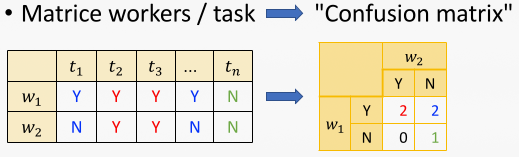
\includegraphics[width=0.7\linewidth]{figures/perc_agr.png}
    \end{figure}
    \noindent
      \begin{minipage}[c]{0.68\linewidth}
          La percentuale di accordo tra due worker è semplice da calcolare con la matrice d confusione: $p=\frac{a+d}{a+b+c+d}$
      \end{minipage}
      \hfill
      \begin{minipage}[c]{0.28\linewidth}
          \centering
          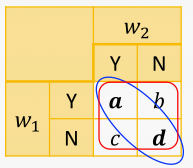
\includegraphics[width=\linewidth]{figures/perc_ag.png}
      \end{minipage}
    \noindent
      \begin{minipage}[t]{0.48\linewidth}
          \textbf{Pro}:
          \begin{itemize}
              \item Facile da calcolare;
              \item Intuitivo;
              \item Consente confronti;
              \item Facilmente estendibile a \textbf{più categorie} (finché si resta in scala nominale).
          \end{itemize}
      \end{minipage}
      \hfill
      \begin{minipage}[t]{0.48\linewidth}
          \textbf{Contro}
          \begin{itemize}
              \item Agreement by chance, accordo casuale tra gli worker (2 cat: 50$\%$, 3 cat: 33$\%$);
              \item Categorie sbilanciate (se worker sanno che 90$\%$ di risposte sono N diranno a loro volta N al 90-100$\%$).
          \end{itemize}
      \end{minipage}
  \subsection{Cohen's kappa (K)}
    Idea: \textbf{migliorare / correggere percent agreement} tenendo conto dell'\textbf{agreement by chence}:
    \begin{itemize}
        \item sempre 2 worker;
        \item sempre scala nominale $K=\frac{p_o-p_e}{1-p_e}$;
        \item $p_o$ è percent agreement osservato;
        \item $p_e$ è percent agreement by chance atteso (calcolato usando dati per stimare probabilità che ogni worker scelga una data categoria).
    \end{itemize}
    \subsubsection{Esempio}
      \begin{figure}[H]
          \centering
          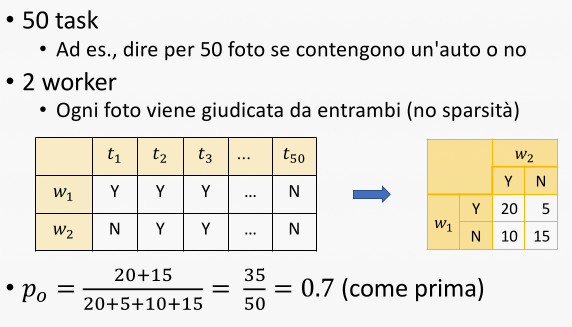
\includegraphics[width=0.6\linewidth]{figures/cohen_1.png}
      \end{figure}
      \noindent
        \begin{minipage}[c]{0.58\linewidth}
          \begin{itemize}
              \item $w_1$ ha detto 25 volte Y (e 25 volte N) $\rightarrow$ $w_1$ ha detto 50\% di volte Y (e 50\% di volte N)
              \item $w_2$ ha detto 30 volte Y (e 20 volte N) $\rightarrow$ $w_1$ ha detto 60\% di volte Y (e 40\% di volte N)
              \item Probabilità che entrambi dicano Y: $p_Y = \frac{a+b}{a+b+c+d} \cdot \frac{a+c}{a+b+c+d} = 0.5 \times 0.6 = 0.3$
              \item Probabilità che entrambi dicano N: $p_N = \frac{c+d}{a+b+c+d} \cdot \frac{b+d}{a+b+c+d} = 0.5 \times 0.4 = 0.2$
              \item $p_e = p_Y + p_N = 0.3 + 0.2 = 0.5$
          \end{itemize}
        \end{minipage}
        \hfill
        \begin{minipage}[c]{0.38\linewidth}
            \centering
            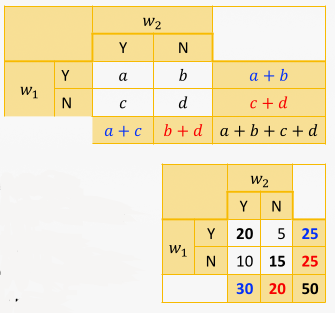
\includegraphics[width=\linewidth]{figures/cohen_2.png}
        \end{minipage}
      Quindi $K=\frac{p_o-p_e}{1-p_e}=\frac{0.7-0.5}{1-0.5}=0.4$ (notare che $K$ può essere $< 0$).
    \subsubsection{Scott's pi}
      Stessa idea di Cohen's kappa, correggendo / normalizzando sulla base dell'accordo casuale. \textbf{ENTRAMBI LIMITATI, SOLO 2 WORKER}.
  \subsection{Fleiss kappa (K)}
    Estende Scott's pi con $m$ worker, scala nominale e un n° di categorie a piacere. Per misurare accordo tra i worker si ricorre a \textbf{pairwise agreement}, considerando tutte le coppie di worker e vedendo quale frazione di coppie è in accordo.
    \subsubsection{Definizione}
      Definizione generale: $K = \frac{\bar{P}-\bar{P}_e}{1-\bar{P}_e}$, come Cohen's kappa ma con pairwise agreement invece di percent agreement.
      \begin{itemize}
          \item $m$: numero di worker;
          \item $n$: numero di task;
          \item $k$: numero di categorie;
          \item $n_{ij}$: numero di worker che hanno assegnato task $i$ alla categoria $j$;
          \item Proporzione di assegmanenti a categoria $j$: $p_j = \frac{1}{nm}\sum_{i=1}^nn_{ij}$;
          \item Somma dei loro quadrati: $\bar{P_e} = \sum_{j=1}^kp_j^2$;
          \item Coppie worker-worker in accordo rispetto a tutte le coppie possibili: $P_i = \frac{2}{m(m-1)}\sum_{j=1}^k\frac{n_{ij}(n_{ij}-1)}{2}$;
          \item Media su tutti gli item: $\bar{P}=\frac{1}{n}\sum_{i=1}^nP_i$.
      \end{itemize}
  \subsection{Sfruttare l'accordo}
    Escludendo i worker che hanno agreement con l'aggregazione inferiore (magari iterativamente), pesarli di meno nell'aggregazione (in caso di media pesata) o utilizzando un modello più sofisticato.
\end{document}
